% =====================================================================
%  An Ablation-Grounded Ensemble for Dermoscopic Skin Lesion Classification
%  Session 5, Part C.
%
%  Every quantitative claim in this file is traceable to an artifact under
%  results/ or to a report under research/*/results/. See Sec. III-G for the
%  frozen-artifact declaration. Do not hand-enter numbers here.
%
%  Build:  pdflatex manuscript && bibtex manuscript && pdflatex manuscript x2
% =====================================================================
\documentclass[journal]{IEEEtran}

\usepackage{graphicx}
\usepackage{amsmath,amssymb}
\usepackage{booktabs}
\usepackage{multirow}
% The appendix checklists run to several pages, so they are longtables. longtable cannot
% break across a two-column page, which is why the appendices switch to \onecolumn.
\usepackage{longtable}
\usepackage{url}
\usepackage[hidelinks]{hyperref}
\usepackage{xcolor}
% Equalises the two columns on the final page. If Overleaf's IEEEtran build ever
% objects, deleting this line and the lone \balance below is the whole fix.
\usepackage{balance}

\graphicspath{{figures/}}

% Shorthand for the escalating-class set, used throughout.
\newcommand{\escset}{\{\textsc{akiec},\,\textsc{bcc},\,\textsc{mel}\}}

\begin{document}

\title{An Ablation-Grounded Ensemble for Dermoscopic\\ Skin Lesion Classification:
Subgroup-Conditional Calibration, Abstention and Conformal Guarantees}

% Single-author submission; the corresponding-author marker is set below. An ORCID iD and
% an IEEE membership grade (\IEEEmembership{Student Member, IEEE}) may be added to the
% \author macro if the author holds them.
\author{Rajrup%
\thanks{Manuscript submitted \today. \emph{(Corresponding author: Rajrup.)}}%
\thanks{The author is with the School of Computing Science and Engineering,
VIT Bhopal University, Kothri Kalan, Madhya Pradesh 466114, India
(e-mail: rajrup.23bai10213@vitbhopal.ac.in).}%
\thanks{Code, the frozen prediction matrices behind every reported number, and the scripts
that regenerate all tables and figures are available at
\url{https://github.com/Rajrup910/Backend-S4D-}.}%
\thanks{This work used the HAM10000 dataset, which is publicly available under CC BY-NC 4.0;
no new human-subjects data were collected.}}

\markboth{IEEE TRANSACTIONS ON MEDICAL IMAGING, VOL.~XX, NO.~X, MONTH~2026}%
{Rajrup: An Ablation-Grounded Ensemble for Dermoscopic Skin Lesion Classification}

\maketitle

% =====================================================================
\begin{abstract}
Reported accuracy on public dermoscopy benchmarks has largely saturated, yet the properties
that decide whether a classifier is deployable --- calibration, knowing when to defer, and
whether its guarantees hold for the patients who need them --- are rarely measured, and almost
never \emph{per subgroup}. We build a seven-class HAM10000 classifier as an ablation ladder
with every component fitted on validation or on $6{,}981$ out-of-fold training predictions,
never on test, and every test quantity from one pass against a pre-registered $19$-item
analysis plan. A uniform soft-vote over six CNN backbones reaches
Macro-F1 $0.7718$; $24$-view test-time augmentation gives $0.7859$ and Dirichlet calibration
$0.8047$, cutting expected calibration error from $0.1575$ to $0.0206$. Ensembling is the only
rung clearing significance (McNemar, Holm-adjusted $p=2.0\times10^{-4}$); five further
combination levers, among them a mixed CNN--transformer ensemble and a $30$-member fold bag,
are all negative, and we report that exhaustion as a result. What remains is subgroup
structure. Marginal conformal coverage at $\alpha=0.10$ attains $90.1\%$ overall, $73.4\%$ on
malignant lesions, and $23.8\%$ on malignant lesions in patients under $40$; class-conditional
calibration lifts that last figure only to $0.57$, while calibrating jointly on age band
$\times$ escalation requirement reaches $0.95$. Escalation sensitivity under $40$ is $0.143$
$[0.030, 0.363]$ against $0.764$ $[0.683, 0.836]$ at $60+$ (difference $-0.621$, Holm
$p<0.001$), and abstention defers only $11\%$ of those misses. A one-parameter age-conditional
rule fitted out-of-fold raises escalation sensitivity from $0.731$ to $0.831$ \emph{overall},
at a Number Needed to Biopsy of $3.0 \rightarrow 6.2$ at a stated $3\%$ reference prevalence
--- but it helps the under-$40$ band least, lifting it only to $0.238$: the blind spot is
mitigated, not closed. Carried frozen to two further
dermoscopic centres ($11{,}982$ BCN-20000 and $2{,}903$ MSKCC images, nothing re-fitted), that
rule again raises under-$40$ escalation sensitivity ($0.279 \rightarrow 0.352$ and $0.333
\rightarrow 0.389$) --- while both pre-registered mechanistic claims fail. The operating point
transports; the explanation does not.
\end{abstract}

\begin{IEEEkeywords}
Skin lesion classification, dermoscopy, model calibration, conformal prediction, selective
classification, ensemble methods, algorithmic fairness, hidden stratification, HAM10000.
\end{IEEEkeywords}

% =====================================================================
\section{Introduction}
\IEEEPARstart{A}{utomated} classification of dermoscopic images has been among the most
visible successes of deep learning in medicine. Since the demonstration that a convolutional
network could match board-certified dermatologists on biopsy-proven lesion
classification~\cite{esteva2017}, the field has converged on a small number of public
benchmarks --- principally the HAM10000 collection~\cite{tschandl2018ham10000} and the ISIC
challenge series~\cite{codella2018isic} --- and on a reporting convention centred on
aggregate discrimination: accuracy, macro-averaged F1, area under the ROC curve.

That convention has outlived its usefulness. On HAM10000 the marginal returns to
architecture are now small and, as we show, statistically unresolvable at the size of a
standard held-out split: the gap between the weakest and strongest backbone we train
($0.7058$ versus $0.7459$ Macro-F1) is not significant under a paired test, and a Vision
Transformer does not beat the best CNN. Meanwhile the properties that decide whether such a
system can be placed in a clinical pathway are usually left unmeasured. A classifier whose
softmax outputs are badly calibrated cannot be composed with a cost model. A classifier with
no abstention mechanism must answer every case, including the ones it has no business
answering. A classifier whose coverage guarantee holds only on average will, in a dataset
where two thirds of the images are ordinary moles, purchase that average from the benign
majority and leave the malignant minority uncovered.

\subsection{Contributions}
This paper is organised around the claim that \emph{deployability is a measurable property},
that measuring it changes which design choices look worthwhile, and that measuring it
\emph{in aggregate} is not enough.

\begin{enumerate}
\item \textbf{An ablation ladder with honest statistics, and a reported exhaustion result.}
We report eleven configurations in two blocks, each with a $1000\times$ lesion-grouped
bootstrap $95\%$ confidence interval, and paired McNemar and DeLong tests within declared
correction families (Sec.~\ref{sec:results-ladder}). We then test five further combination
levers --- adding two transformer members, greedy member selection, global and per-class
prior correction, and a $30$-member fold-bagged ensemble --- and report all five as negative
(Sec.~\ref{sec:results-exhaustion}). Macro-F1 $0.8047$ is the ceiling of these checkpoints
under any post-hoc recombination we could find.
\item \textbf{A calibration analysis that is resolved per subgroup.} The soft-vote ensemble
is systematically \emph{under}confident, the opposite of the single-network result the
calibration literature reports, which is why a one-parameter temperature is the wrong remedy
here. We further show the miscalibration is not uniform across age bands, and that a single
global Dirichlet map leaves residuals of \emph{opposite sign} in different bands
(Sec.~\ref{sec:results-calibration}) --- the empirical case for group-wise
calibration~\cite{hebertjohnson2018multicalibration}.
\item \textbf{A selective-classification analysis} with out-of-fold-fitted abstention
thresholds and a risk--coverage characterisation, including the negative result that
feature-space (Mahalanobis) and disagreement-based scores rank in-distribution errors
\emph{worse} than the plain probability margin --- and the paired positive result that the
same Mahalanobis score separates in-distribution dermoscopy from out-of-distribution
smartphone photography at AUROC $0.913$, which is the shift it was designed
for~\cite{ovadia2019shift} (Secs.~\ref{sec:results-selective},~\ref{sec:results-external}).
\item \textbf{A conformal analysis showing that class-conditional coverage is not enough
either.} Marginal coverage is the wrong guarantee for an imbalanced screening
problem~\cite{vovk2012conditional}; we show that even Mondrian class-conditional calibration
leaves the under-$40$ malignant subgroup materially under-covered, and that calibrating on
(age band $\times$ escalation requirement) --- an instance of equalised
coverage~\cite{romano2020equalized} --- repairs it. We formalise the \emph{False Reassurance
Rate} as the primary conformal endpoint, report it with intervals, and report the $\alpha$
required to bound it rather than pre-committing to a bound
(Sec.~\ref{sec:results-conformal}).
\item \textbf{A documented, mechanistically probed and priced subgroup failure.} We report an
age-stratified escalation-sensitivity collapse that no aggregate metric in this paper
reveals, characterise it as a confidently-wrong failure, and separate how much of it is a
\emph{decision rule} discarding available signal from how much is genuinely weaker ranking
--- finding, on test, that it is both. We then supply a one-parameter mitigation fitted
out-of-fold, price it in Number Needed to Biopsy at a stated reference prevalence, and
measure whether it is orthogonal to abstention, reporting the band in which it is not
(Secs.~\ref{sec:results-fairness},~\ref{sec:results-utility}).
\item \textbf{An external evaluation on smartphone clinical photography.} The calibrated
ensemble, the frozen calibration map and the frozen age-conditional rule are applied
unmodified to all $2{,}106$ PAD-UFES-20 images, with a Fitzpatrick skin-tone slice in which
the missing-label artefact is separated from the skin-tone signal rather than pooled with it,
and a decomposition separating how much of the transfer collapse is prior shift (recoverable
in principle) from how much is optical (not) --- including the negative result that the
deployable, label-free version of that correction makes matters significantly worse
(Sec.~\ref{sec:results-external}).
\item \textbf{A pre-registered same-modality replication at two further centres, reported
against its own contingency.} The frozen system is carried to $11{,}982$ BCN-20000 and
$2{,}903$ MSKCC dermoscopy images with nothing re-fitted, under a plan that named both its
claims and what to do if they failed. Both failed --- escalation-mass AUC is not
cohort-invariant, and under-$40$ sensitivity tracked the training prior's age skew in reverse
--- while the mitigation itself reproduced at every centre. We report the separation between a
transportable operating point and a non-transportable mechanism as the result, rather than
retiring the hypothesis quietly or rescuing it post hoc (Sec.~\ref{sec:results-battery}).
\item \textbf{A frozen analysis plan and a single test read.} Every test quantity added in
this round --- two new rungs, the age rule, NNB, FRR, bipartite coverage, intersectional
cells, attribution --- was named, defined and hashed into a pre-registered plan
\emph{before} the split was touched, and emitted by one pass that refuses to compute anything
the plan does not name (Sec.~\ref{sec:frozen}).
\end{enumerate}

We also report, deliberately, the design choices that did \emph{not} work, including one
--- a ridge stacking ensemble --- that would have produced our best headline number had we
been willing to select it on the test set. We were not; Sec.~\ref{sec:results-ladder}
explains why that matters.

% =====================================================================
\section{Related Work}

\textbf{Backbones and the imbalance they hide.} Convolutional baselines on HAM10000 and ISIC
are well established~\cite{esteva2017,codella2018isic,tschandl2018ham10000}, and the
architectural frontier has moved through residual~\cite{he2016resnet},
densely-connected~\cite{huang2017densenet}, compound-scaled~\cite{tan2019efficientnet} and
modernised-convolutional~\cite{liu2022convnext} designs, and more recently to hierarchical
Vision Transformers~\cite{liu2022swinv2,tu2022maxvit}. Reported gains between these families
on a single benchmark split are typically one to three F1 points --- which, as our confidence
intervals show, is smaller than the sampling variation of the split itself. What the leader
board hides is that HAM10000 is dominated by melanocytic nevi ($\sim67\%$ of images), so
accuracy is an actively misleading selection criterion. The standard remedies are
re-weighting by effective number of samples~\cite{cui2019classbalanced}, margin-based losses
such as LDAM-DRW~\cite{cao2019ldam}, asymmetric focal variants~\cite{ridnik2021asl}, and the
post-hoc route of logit adjustment by the label prior~\cite{menon2021logitadjust}, whose
probabilistic form dates to prior-shift correction for changing class
priors~\cite{saerens2002adjusting}. We train LDAM-DRW and ASL variants of our strongest
backbone and find neither improves on the cross-entropy baseline under effective-number
weighting (Sec.~\ref{sec:results-ladder}); we report logit adjustment as a negative result
and explain the null mechanistically in Sec.~\ref{sec:results-exhaustion}, and we report the
same family's label-free cousin failing under real prior shift in
Sec.~\ref{sec:results-external}.

\textbf{Calibration, uncertainty and abstention.} Modern single networks are systematically
overconfident~\cite{guo2017calibration}; temperature scaling is the standard one-parameter
remedy, and matrix and Dirichlet scaling~\cite{kull2019dirichlet} generalise it to full
class-conditional recalibration. Our soft-vote ensemble is miscalibrated in the \emph{opposite}
direction (Sec.~\ref{sec:results-calibration}), which is why the one-parameter remedy is not
the right one here. All of these are \emph{marginal} notions. Group-wise notions ---
multicalibration~\cite{hebertjohnson2018multicalibration} and its relatives --- require the
property to hold within identifiable subpopulations, and our per-band results are a direct
empirical argument for adopting one: a globally well-calibrated map can be, and here is,
simultaneously under- and over-confident in different age bands. Selective classification has
a long history~\cite{elyaniv2010selective,geifman2017selectivenet}, with deep-ensemble
disagreement~\cite{lakshminarayanan2017deepensembles} and Mahalanobis feature
distance~\cite{lee2018mahalanobis} as common uncertainty signals. That the latter two
underperform the probability margin on an in-distribution test split is consistent with their
stated purpose --- they are shift detectors, and there is no shift there --- and we confirm
the converse externally.

\textbf{Conformal prediction and whose coverage it is.} Split conformal
prediction~\cite{vovk2005algorithmic,angelopoulos2023gentle} converts any score into
finite-sample coverage guarantees. LAC~\cite{sadinle2019lac} minimises set size;
APS~\cite{romano2020aps} and RAPS~\cite{angelopoulos2021raps} trade size for conditional
validity. The distinction between marginal and class-conditional (Mondrian) coverage is well
known in statistics~\cite{vovk2012conditional} but is, in our reading, under-emphasised in
medical imaging, where it is precisely the clinically relevant distinction. Conditioning on a
clinically salient attribute rather than on the label --- equalised coverage --- is due to
Romano \emph{et al.}~\cite{romano2020equalized}; our bipartite (age band $\times$ escalation
requirement) calibrator is an instance of their construction, and we cite it as such rather
than presenting it as new.

\textbf{Hidden stratification, and our delta over it.} The failure mode this paper is
ultimately about has a name. Oakden-Rayner \emph{et al.}~\cite{oakdenrayner2020hidden} define
\emph{hidden stratification} as the situation in which a clinically meaningful subclass is
systematically mishandled while aggregate metrics stay healthy, and show the effect is common,
large and invisible to the field's reporting conventions. Seyyed-Kalantari
\emph{et al.}~\cite{seyyedkalantari2021underdiagnosis} give the closest prior result: chest
radiograph classifiers that underdiagnose historically underserved groups, again with no
aggregate signal. The mechanism is a shortcut in the sense of Geirhos
\emph{et al.}~\cite{geirhos2020shortcut}, of which the radiograph-site confound of Zech
\emph{et al.}~\cite{zech2018confounding} is the canonical medical instance; ``young patient,
therefore nevus'' is a textbook example, and the training prior we report in
Sec.~\ref{sec:results-fairness} is its source. The skin-tone axis of this literature is the
better documented one~\cite{daneshjou2022disparities}, with Fitzpatrick-labelled
corpora~\cite{groh2021fitzpatrick17k} built to measure it; HAM10000 carries no Fitzpatrick
labels, and Sec.~\ref{sec:limitations} explains why we decline to approximate them from image
statistics, measuring that axis externally on PAD-UFES-20~\cite{pacheco2020padufes} instead.
The age-stratified failure we report appears less discussed, despite being far larger in our
data. Our contribution over this lineage is specific. That work establishes that hidden
stratification exists and evades aggregate metrics. We additionally (i) \emph{measure the
mechanism}, separating a decision rule that discards available signal from a genuine loss of
ranking ability, using a threshold-free within-band AUC; (ii) show that the standard safety
mechanisms --- abstention, calibration and conformal sets --- are themselves inoperative in
the affected subgroup, which is stronger than saying the classifier is worse there; (iii)
supply a mitigation with a priced clinical cost; and (iv) carry that mitigation, frozen, to
two further centres and report what does and does not survive the move. The mitigation is a
group-specific decision threshold, exactly the post-processing construction of Hardt
\emph{et al.}~\cite{hardt2016equality}. We select it by expected clinical cost under a
per-band specificity floor rather than by their formal target of equality of opportunity, and
say so; adopting equality of opportunity directly is the cleaner objective and is left as
stated future work (Sec.~\ref{sec:limitations}).

% =====================================================================
\section{Materials and Methods}
\label{sec:methods}

Fig.~\ref{fig:architecture} summarises the complete system. The ordering of this section
follows the order in which components are fitted, which is also the order of the ablation
ladder in Sec.~\ref{sec:results-ladder}.

\subsection{Data and splits}
All experiments use HAM10000~\cite{tschandl2018ham10000}: $10{,}015$ dermoscopic images of
$7{,}470$ distinct lesions, labelled with the seven diagnostic categories in
Table~\ref{tab:classes}. Because the collection contains multiple images of the same lesion,
an image-level split leaks: near-duplicate views of one lesion would appear on both sides.
We therefore split by \texttt{lesion\_id} at a $70/15/15$ ratio, stratified by diagnosis,
giving $6{,}981$ training images ($5{,}229$ lesions), $1{,}532$ validation images ($1{,}120$
lesions) and $1{,}502$ test images ($1{,}121$ lesions). A machine-checked assertion confirms
that no lesion identifier appears in more than one split; this assertion is re-run by every
downstream script, including the inner cross-validation folds used for stacking.

\begin{table}[t]
\centering
\caption{The seven HAM10000 classes, their malignancy tier, and test-split support.
Starred tiers form the escalating set $\escset$, the positive class for the binary
screening metrics. Note the imbalance: \textsc{nv} alone is $66.8\%$ of the test split,
while \textsc{df} and \textsc{vasc} together are $2.7\%$.}
\label{tab:classes}
\begin{tabular}{llcr}
\toprule
Code & Diagnosis & Tier & Test $n$ \\
\midrule
\textsc{akiec} & Actinic keratosis / intraep.\ ca. & premalignant$^\ast$ & 52 \\
\textsc{bcc}   & Basal cell carcinoma              & malignant$^\ast$    & 71 \\
\textsc{bkl}   & Benign keratosis-like lesion      & benign              & 167 \\
\textsc{df}    & Dermatofibroma                    & benign              & 20 \\
\textsc{mel}   & Melanoma                          & malignant$^\ast$    & 167 \\
\textsc{nv}    & Melanocytic nevus                 & benign              & 1004 \\
\textsc{vasc}  & Vascular lesion                   & benign              & 21 \\
\midrule
\multicolumn{3}{l}{Total} & 1502 \\
\bottomrule
\end{tabular}
\end{table}

\subsection{External cohort}
\label{sec:external-data}
For the external evaluation of Sec.~\ref{sec:results-external} we use all $2{,}106$ images of
PAD-UFES-20~\cite{pacheco2020padufes}, a smartphone clinical-photography cohort covering six of
the seven HAM10000 categories, of which $1{,}302$ carry a Fitzpatrick skin-type label. Nothing
is fitted on PAD: the six backbones, the ensemble, the Dirichlet map and the age-conditional
rule are all applied exactly as frozen on HAM10000. PAD's escalating prevalence of
approximately $77\%$ is the inverse of HAM10000's $19\%$, which is central to how its results
must be read and is discussed where they are reported.

Because a change of imaging modality confounds every explanation at once, the replication of
Sec.~\ref{sec:results-battery} uses two further \emph{dermoscopic} centres from
ISIC-2019~\cite{combalia2019bcn20000, codella2018isic}: BCN-20000 and MSKCC, held in a
lesion-grouped split of $14{,}885$ records. Squamous-cell carcinoma is excluded by
pre-registration, because it has no HAM10000 counterpart and the frozen head cannot emit it;
that removes $431$ BCN-20000 images and leaves $11{,}982$ against MSKCC's $2{,}903$. MSKCC's
label space contains only \textsc{nv}, \textsc{mel} and \textsc{bkl}, so seven-class Macro-F1
is undefined there and we report escalation-focused metrics for that centre instead. Both
cohorts are scored by the same six frozen HAM10000-only checkpoints under the same $24$-view
test-time augmentation, combined by the same uniform vote and mapped by the same
HAM10000-out-of-fold Dirichlet calibrator; the per-band $\lambda$ is likewise carried across
unchanged. No parameter anywhere in this paper is fitted on BCN-20000 or MSKCC.

The external analysis was pre-registered before the two cohorts were scored. The plan names
its endpoints, its five-member Holm family, the interval method for each quantity, and a
contingency for each way a claim could fail; it is stored with its SHA-256 digest alongside
the frozen prediction matrices, together with its superseded first version and a numbered
record of the seven deviations between them. The most consequential deviation is worth
stating in the text: version~1 named the wrong out-of-fold Dirichlet fit. Three exist in this
project, they differ by up to $0.18$ in the calibration weight matrix, and only one of them is
the map the system actually deploys. Every external number here uses the deployed map, loaded
through a single accessor that no analysis script is permitted to bypass.

\subsection{The age-conditional escalation rule}
\label{sec:agerule}
Sec.~\ref{sec:results-fairness} shows that in the under-$40$ band the escalating-class
probability mass carries usable signal that the $\arg\max$ rule discards. The mitigation is
therefore a decision rule, not a retrained model, and we deliberately keep it to one
parameter per band. Writing $\mathcal{E}$ for the escalating set and $b(x)$ for the patient's
age band, the rule predicts
\begin{equation}
\hat{y}(x) \;=\; \arg\max_{c}\;\bigl(p_c(x) + \lambda_{b(x)}\,\mathbf{1}[c \in \mathcal{E}]\bigr),
\label{eq:lambda}
\end{equation}
which is equivalent to applying per-class thresholds $\theta_c = -\lambda_b$ on the escalating
classes and $0$ elsewhere. This is the group-specific threshold construction of Hardt
\emph{et al.}~\cite{hardt2016equality}, applied to an age band rather than to a protected
attribute in their sense.

One scalar per band is a deliberate choice over a per-band seven-vector: a $13$-point
$\times$ $7$-class threshold grid fitted on $22$ positives would overfit, whereas one
parameter on $64$ is defensible. Each $\lambda_b$ is chosen by exhaustive search over a
$61$-point grid to minimise expected clinical cost under the same cost matrix used for the
cost-sensitive thresholds, subject to a per-band escalation-specificity floor of $0.85$, with
ties resolved towards the smaller $\lambda$ so that the operating point referring fewer
patients wins. A band with fewer than $30$ true escalating cases does not get its own
$\lambda$ and falls back to the pooled value; the gate counts positives rather than group
size, because a band of $400$ nevi with eight malignancies says nothing about where its
escalation boundary belongs beyond what those eight cases say. That gate is why the rule is
fitted on OOF and nowhere else: validation has $22$ escalating under-$40$ cases and OOF has
$64$.

Fitting uses cross-fitted Dirichlet-calibrated OOF probabilities, so the calibrator has not
seen the rows its own $\lambda$ is tuned on. The frozen values are $\lambda_{<40}=0.26$
(bootstrap CI $[0.00, 0.61]$), $\lambda_{40\text{--}59}=0.74$, $\lambda_{60+}=0.33$, and a
pooled $0.65$ for the small number of records with no recorded age. The under-$40$ interval
touching zero is the honest reading of $64$ positives and is the reason this rung was
pre-registered two-sided.


\textit{The remaining apparatus --- the out-of-fold protocol, metric definitions, backbone training, ensembling, test-time augmentation and calibration, selective prediction and conformal set construction, and the statistical protocol with its frozen-artifact declaration --- is specified in Appendix~\ref{app:extmethods}. It is held back for length, not because it is optional: every number in this paper depends on it.}
\section{Results}

\begin{figure*}[t]
\centering
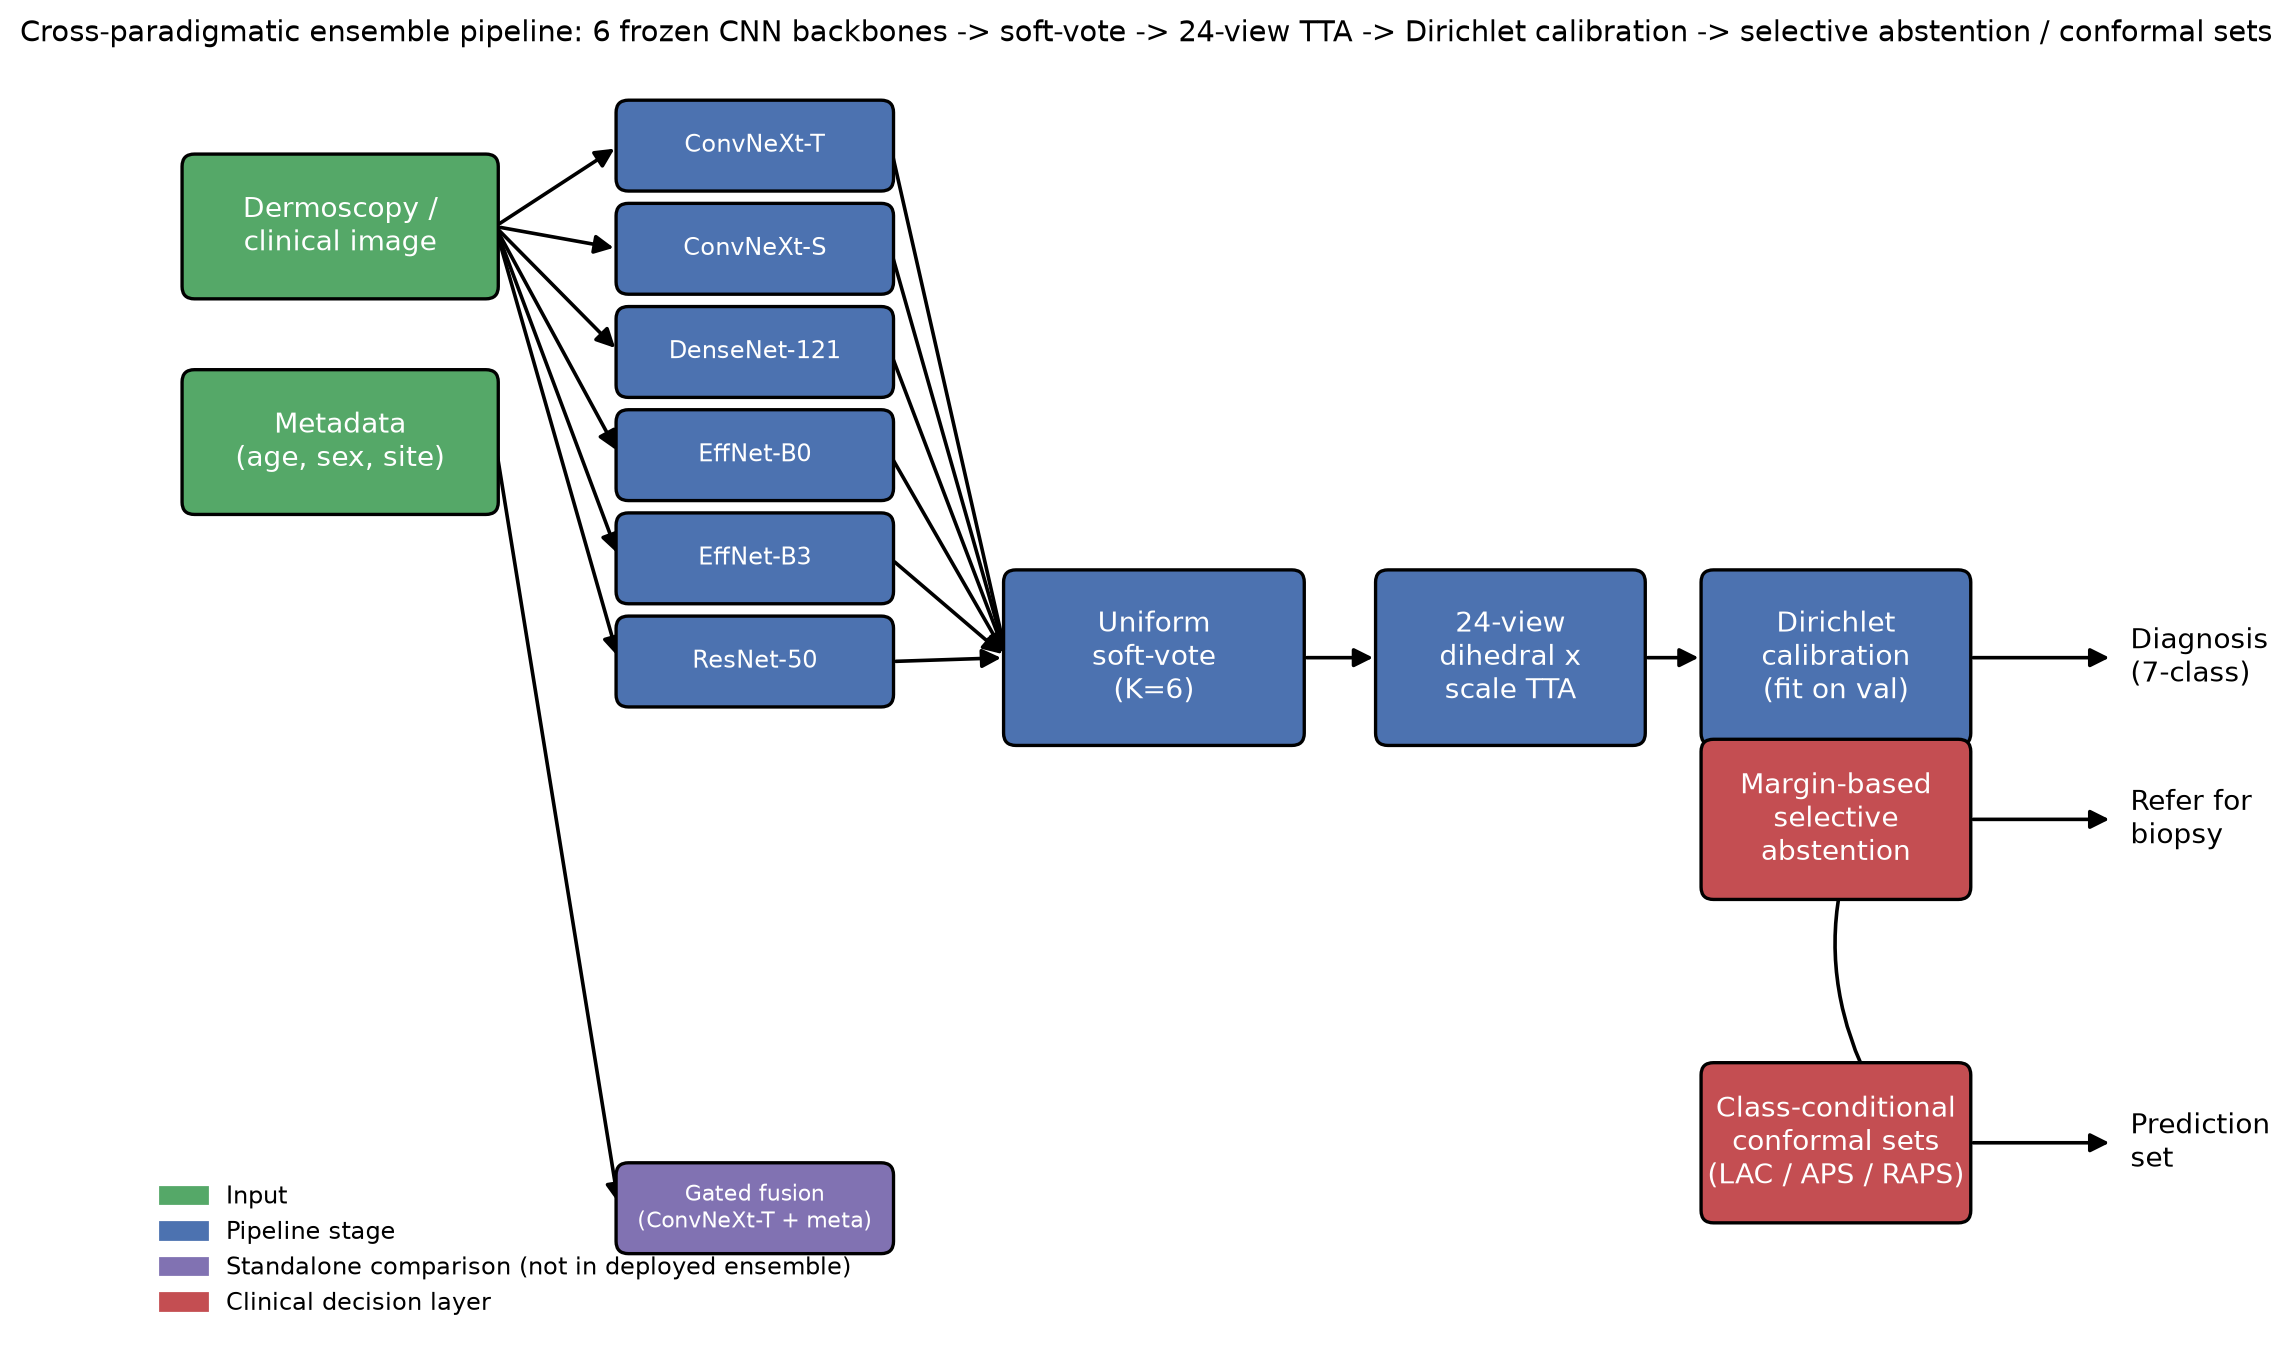
\includegraphics[width=0.74\textwidth]{figure1_architecture.png}
\caption{System overview. Six frozen CNN backbones produce probability vectors that are
pooled by uniform soft-vote over $24$ deterministic TTA views, recalibrated by a Dirichlet
map fitted on validation, and passed to two parallel decision layers: a margin-based
abstention gate and a Mondrian class-conditional conformal set constructor. Every fitted
component downstream of the backbones is fitted on validation data only.}
\label{fig:architecture}
\end{figure*}

\subsection{Calibration and decision rules}
\label{sec:results-calibration}

\begin{figure*}[t]
\centering
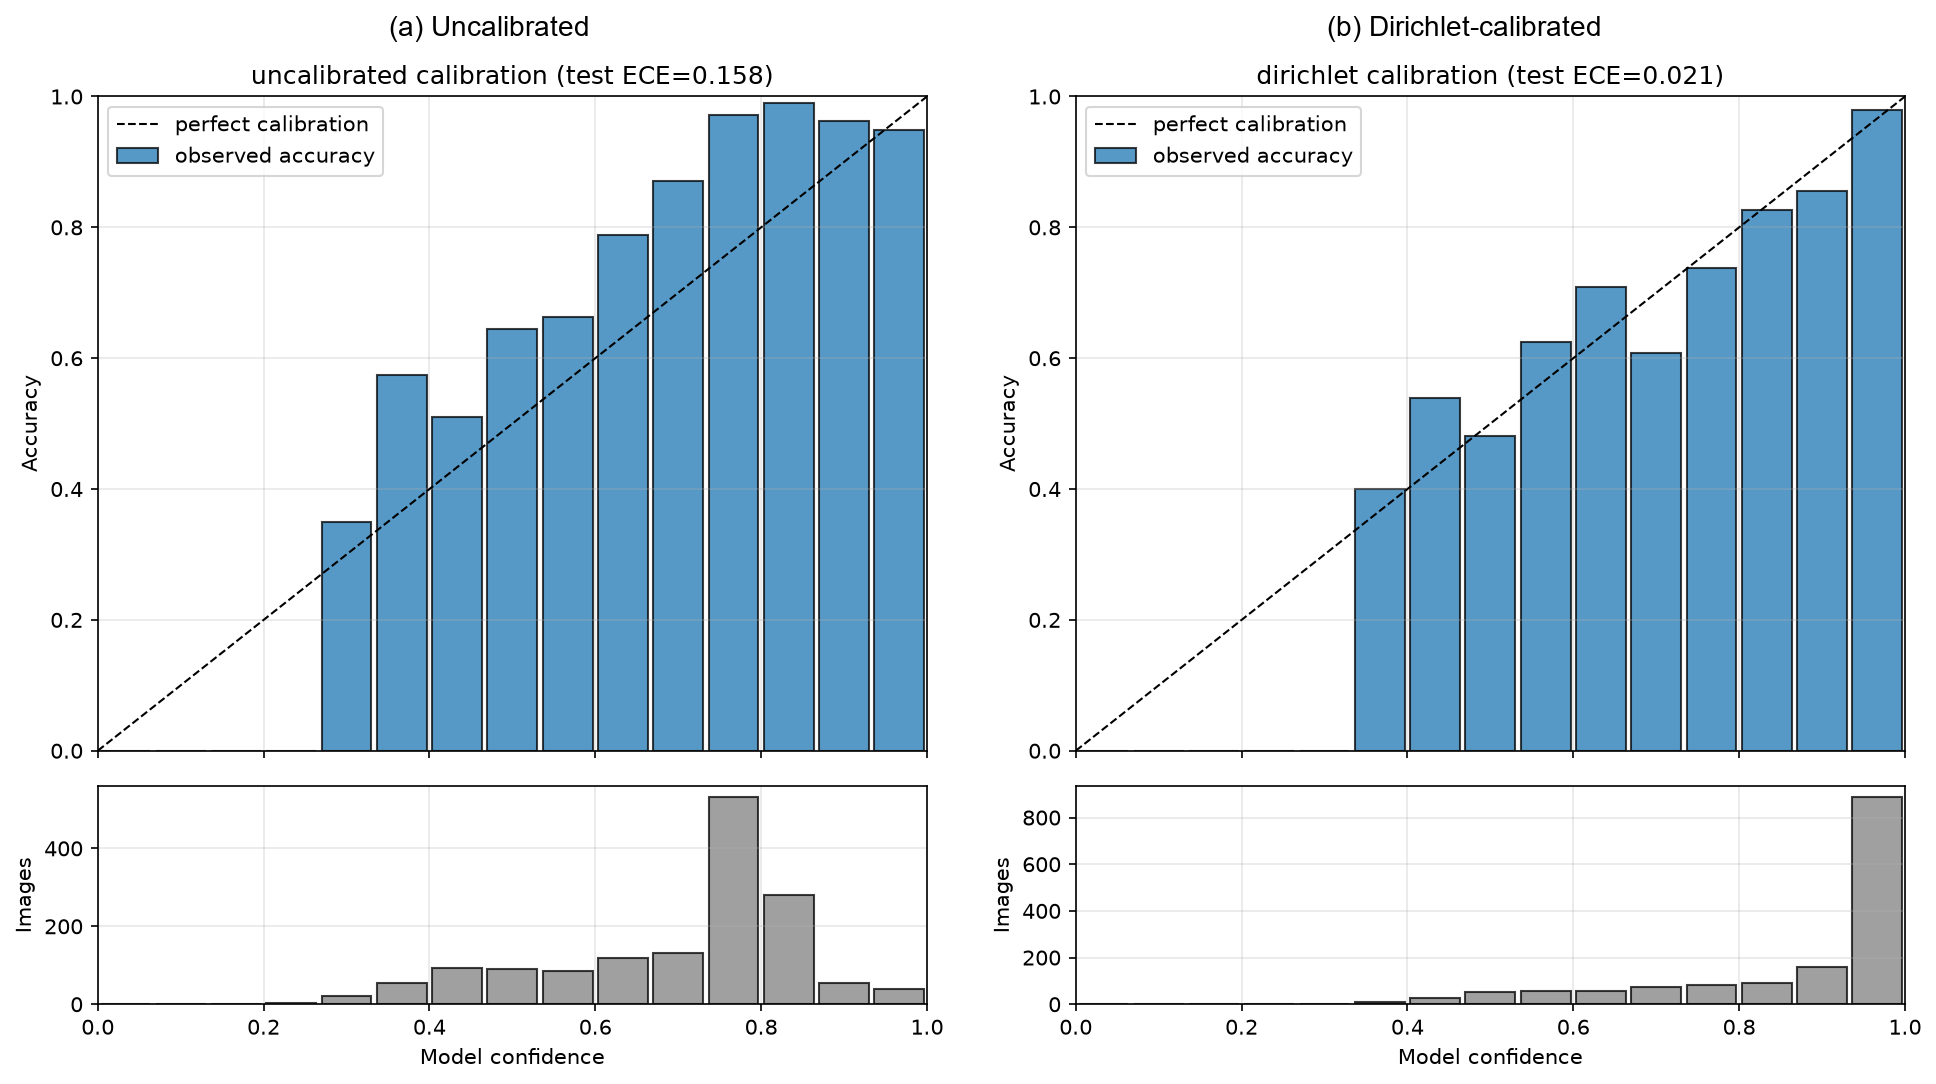
\includegraphics[width=0.72\textwidth]{figure2_reliability.png}
\caption{Reliability diagrams for the six-CNN soft-vote ensemble before (a) and after
(b) Dirichlet calibration, fitted on validation and evaluated on the held-out test split.
Test ECE falls from $0.1575$ to $0.0206$. Note the direction: the uncalibrated bars sit
\emph{above} the diagonal almost everywhere, so accuracy exceeds stated confidence. Soft-vote
averaging over six members dilutes the peak probability, leaving the ensemble
systematically \emph{under}confident --- the opposite of the single-network overconfidence
usually reported.}
\label{fig:reliability}
\end{figure*}

The uncalibrated ensemble is substantially miscalibrated, with test ECE $0.1575$
(Fig.~\ref{fig:reliability}), but not in the direction the calibration literature leads one
to expect. Its mean confidence is $0.7048$ against an accuracy of $0.8609$ --- a signed gap
of $-0.156$ that accounts for essentially all of the ECE. The ensemble is systematically
\emph{under}confident. The mechanism is soft-voting itself: averaging six probability
vectors that disagree about the runner-up class pulls the maximum probability down, so the
aggregate is more hedged than any of its members. Single backbones show the same sign but
much weaker (ConvNeXt-Tiny: confidence $0.7606$, accuracy $0.8296$). This matters for method
choice, because it is a class-dependent distortion rather than a uniform sharpening, and a
one-parameter temperature cannot express it. Ranked by validation ECE, Dirichlet calibration
wins
($0.0201$ validation, $0.0206$ test), ahead of matrix scaling ($0.0263$ / $0.0279$) and
temperature scaling ($0.0338$ / $0.0322$). Temperature scaling leaves the argmax unchanged
and therefore leaves Macro-F1 at $0.7718$; matrix scaling degrades it to $0.7417$; Dirichlet
improves it to $0.7907$ on the plain ensemble and to $0.8047$ once combined with TTA.

\textbf{The miscalibration is not uniform across age bands, and one global map cannot express
that.} Aggregate ECE conceals structure. Table~\ref{tab:bandcal} slices confidence and
accuracy by age band on the test split, before and after the Dirichlet map, for the deployed
TTA ensemble; the table carries its own aggregate row so every entry shares a base system.
Two things are visible. First, the bands are miscalibrated by different amounts: the
uncalibrated signed gap ranges from $-0.197$ to $-0.105$, and per-band ECE from $0.198$ to
$0.113$, an ECE spread of $0.084$ hidden inside an aggregate of $0.158$. Second, and more
consequentially, \emph{one global affine map leaves residuals of opposite sign in different
bands}: after Dirichlet calibration the $40$--$59$ band remains under-confident at $-0.023$
while the $60+$ band is pushed into over-confidence at $+0.034$, so an aggregate signed gap of
$+0.004$ is the average of two errors pointing in opposite directions. The band spread in ECE
narrows from $0.084$ to $0.029$ but does not close.

\begin{table}[t]
\centering
\caption{Per-age-band calibration of the deployed TTA ensemble on the test split, before and
after the global Dirichlet map. Signed gap is mean confidence minus accuracy, so negative is
\emph{under}confidence. The aggregate row is computed on the same base system as the band
rows. Note the sign disagreement after calibration: no single global affine map can be
simultaneously correct for a band it must sharpen and a band it must soften.}
\label{tab:bandcal}
\begin{tabular}{lrcccc}
\toprule
& & \multicolumn{2}{c}{Uncalibrated} & \multicolumn{2}{c}{Dirichlet} \\
\cmidrule(lr){3-4}\cmidrule(lr){5-6}
Band & $n$ & Signed gap & ECE & Signed gap & ECE \\
\midrule
$<40$      & 290  & $-0.163$ & $0.167$ & $+0.015$ & $0.046$ \\
$40$--$59$ & 671  & $-0.197$ & $0.198$ & $-0.023$ & $0.034$ \\
$60+$      & 532  & $-0.105$ & $0.113$ & $+0.034$ & $0.063$ \\
\midrule
All        & 1502 & $-0.158$ & $0.158$ & $+0.004$ & $0.017$ \\
\bottomrule
\end{tabular}
\end{table}

We are careful about which part of this replicates. The \emph{sign disagreement} does: on
validation, out-of-fold and test alike, the $60+$ band ends over-confident after calibration
($+0.030$, $+0.041$, $+0.034$) while at least one younger band remains under-confident. The
\emph{ranking} does not. On the better-powered out-of-fold split the under-$40$ band is the
most under-confident of the three ($-0.229$ against $-0.190$ and $-0.119$) and simultaneously
the most ``accurate'' at $0.930$, because it is dominated by easy nevi --- an attractive
finding that we set out expecting to confirm. On test the largest uncalibrated gap belongs to
the $40$--$59$ band instead. We therefore report the sign disagreement as a finding and the
ordering as unreplicated: \emph{which} band is worst calibrated is not stable at these
counts; that a single global map leaves opposite-signed residuals across bands is.

That is the empirical case for group-wise rather than global recalibration ---
multicalibration in the sense of H\'ebert-Johnson
\emph{et al.}~\cite{hebertjohnson2018multicalibration} --- and it is the point at which this
paper's calibration thread and its fairness thread turn out to be one thread.

\textbf{Calibration and screening sensitivity pull in opposite directions.} This is the most
important caveat attached to rung A7 and we state it plainly: while Dirichlet calibration
raises Macro-F1 from $0.7859$ to $0.8047$, it \emph{lowers} escalation sensitivity from
$0.7862$ to $0.7310$, increasing missed serious cases from $62$ to $78$. Recalibration
redistributes probability mass towards the majority \textsc{nv} class, which is correct in a
proper-scoring sense and harmful in a screening sense. A deployment that cares about missed
melanomas more than about balanced class-wise F1 should not adopt A7 without also adopting a
decision rule that restores sensitivity.

\textbf{Cost-sensitive thresholding restores sensitivity but is redundant with abstention.}
Per-class thresholds fitted on Dirichlet-calibrated validation probabilities subject to a
specificity floor of $0.85$ raise escalation sensitivity from $0.7310$ to $0.8621$ and cut
missed serious cases from $78$ to $40$, at a cost of $-0.062$ Macro-F1. We therefore report
it as a decision-rule sub-analysis on the sensitivity axis, not as a rung on the Macro-F1
ladder. Moreover the two mechanisms overlap almost exactly: of the $168$ predictions the cost
rule changes at full coverage, $128$ remain at $5\%$ abstention, $80$ at $10\%$, $27$ at
$15\%$, and \emph{zero} at $20\%$. Every prediction the cost rule alters is a low-margin
case, and by a $20\%$ abstention rate all of them have already been referred. The two
configurations converge to the identical Macro-F1 of $0.8957$ at that operating point ---
a coincidence of value that is in fact a structural identity.

Decision curve analysis~\cite{vickers2006dca} is reported in
Sec.~\ref{sec:results-battery} rather than here. An earlier version of this paper carried a
curve comparing the ensemble with its best single member and with a treat-all policy; that
comparison is already settled, and settled more precisely, by the ablation ladder. The
clinically live question is whether the escalation rule of Sec.~\ref{sec:agerule} earns the
extra referrals it buys, and Fig.~\ref{fig:dca} answers that one.

\subsection{Conformal prediction}
\label{sec:results-conformal}

\begin{table}[t]
\centering
\caption{Conformal prediction at $\alpha = 0.10$. \emph{Serious} restricts coverage to
lesions truly in $\escset$. \emph{False reassurance} counts malignant lesions whose
prediction set contained no escalating class at all. A marginal guarantee is satisfied by
every row in the first block, and is clinically inadequate in all of them.}
\label{tab:conformal}
\begin{tabular}{llcccr}
\toprule
Score & Calibration & Marg. & Serious & Size & False reas. \\
\midrule
LAC  & marginal & 0.904 & 0.748 & 1.08 & 63 \\
APS  & marginal & 0.919 & 0.838 & 1.34 & 39 \\
RAPS & marginal & 0.900 & 0.752 & 1.12 & 63 \\
\midrule
LAC  & class-cond. & 0.900 & 0.914 & 2.16 & 17 \\
APS  & class-cond. & 0.931 & 0.945 & 2.06 & 11 \\
RAPS & class-cond. & 0.927 & \textbf{0.941} & 2.68 & \textbf{6} \\
\bottomrule
\end{tabular}
\end{table}

Table~\ref{tab:conformal} contains what we consider the paper's sharpest methodological
result. At $\alpha=0.10$, LAC under marginal calibration attains $90.4\%$ empirical coverage
--- the guarantee holds exactly as advertised --- while covering only $74.8\%$ of genuinely
malignant lesions, and producing $63$ prediction sets for malignant lesions that contain no
escalating class whatsoever. The marginal average is being financed by the $67\%$ of cases
that are ordinary moles. A clinician handed such a set for a melanoma would receive a
confident, well-calibrated, formally valid, and entirely wrong shortlist.

Mondrian class-conditional calibration repairs this. Coverage on serious cases rises to
$91.4\%$ (LAC), $94.5\%$ (APS) and $94.1\%$ (RAPS), and false reassurances fall to $17$,
$11$ and $6$ respectively. The price is shortlist length: LAC's mean set size rises from
$1.08$ to $2.16$ and its singleton rate falls from $91.5\%$ to $18.6\%$, meaning the system
commits to a single diagnosis far less often. We consider this trade clearly worth making.
A two-item shortlist that contains the melanoma is clinically useful; a confident singleton
that does not is worse than no output. Among the validation-calibrated configurations, which
are the ones carrying an exact finite-sample guarantee, the best by the clinical criterion of
false reassurances is RAPS with class-conditional calibration at $\alpha=0.10$; the
subgroup-conditional results below revise that recommendation once the guarantee is relaxed.
Fig.~\ref{fig:conformal} shows the per-class coverage profile under both calibration schemes.

At $\alpha = 0.05$ the same qualitative pattern holds, but a sample-size limit binds: a
class-conditional threshold requires $\lceil (n+1)(1-\alpha) \rceil \le n$ calibration points
of that class, and \textsc{df} and \textsc{vasc} have only $11$ each in the calibration half.
No finite threshold for those classes carries the guarantee, so they are conservatively
included in essentially every prediction set --- six degenerate cells in total. Part of the
mean set size at $\alpha=0.05$ is therefore calibration-set scarcity rather than genuine model
uncertainty. The remedy is more calibration data for rare classes, not a smaller $\alpha$, and
the out-of-fold protocol of Sec.~\ref{sec:oof} supplies it: $3{,}468$ calibration rows instead
of $762$, a rarest-class count of $45$ instead of $11$, and \emph{zero} degenerate cells at
$\alpha=0.05$ (Table~\ref{tab:oof_vs_val}). What it does not supply is the theorem, for the
exchangeability reason given in Sec.~\ref{sec:methods}; the OOF-calibrated results below are
audited empirically against nominal $1-\alpha$ and are never asserted to be guaranteed.

\textbf{Class-conditional coverage is necessary and still not sufficient.} The natural
question, once the marginal-versus-conditional distinction is in hand, is whether
class-conditional coverage is enough. It is not. Table~\ref{tab:bipartite} adds a column that
no conformal evaluation we are aware of reports: coverage restricted to \emph{escalating
lesions in patients under $40$}, the subgroup Sec.~\ref{sec:results-fairness} shows the
classifier fails. Under marginal calibration at $\alpha=0.10$ that coverage is $0.238$ for
LAC and $0.143$ for RAPS --- against nominal $0.90$. Mondrian class-conditional calibration,
which repairs the aggregate malignant coverage to $0.886$--$0.903$, lifts the under-$40$
malignant figure only to $0.571$--$0.667$. Conditioning on the label fixes the label
imbalance and leaves the \emph{patient} imbalance untouched.

Calibrating on the pair (age band, escalation requirement) --- the bipartite scheme of
Sec.~\ref{sec:methods}, an instance of equalised coverage~\cite{romano2020equalized} ---
closes it: $0.952$ for LAC and $0.857$ for RAPS at $\alpha=0.10$, with aggregate serious
coverage \emph{also} at or above the class-conditional value and a mean set size that is
\emph{smaller}, not larger ($1.26$ against $1.28$ for LAC). The usual size-for-validity trade
does not bind here, because six well-populated cells estimate their quantiles more sharply
than seven cells two of which are nearly empty.

\begin{table}[t]
\centering
\caption{Conformal calibration schemes on the test split, out-of-fold calibrated. ``Serious''
restricts coverage to lesions truly in $\escset$; ``$<$40 ser.'' restricts it further to
those in patients under $40$ ($n=21$). FRR is the false reassurance rate of
Eq.~\eqref{eq:frr} with an exact $95\%$ interval. Coverage is audited against nominal
$1-\alpha$, not guaranteed: the out-of-fold calibration scores come from five fold models and
the test scores from the full-train ensemble, so no exact finite-sample guarantee transfers
(Sec.~\ref{sec:methods}).}
\label{tab:bipartite}
\setlength{\tabcolsep}{4pt}
\begin{tabular}{llccccc}
\toprule
$\alpha$ & Calibration & Cov. & Serious & $<$40 ser. & FRR [95\% CI] & Size \\
\midrule
\multicolumn{7}{l}{\textit{LAC}} \\
0.10 & marginal     & 0.901 & 0.734 & 0.238 & 0.228 [0.169, 0.288] & 1.08 \\
0.10 & class-cond.  & 0.875 & 0.886 & 0.571 & 0.079 [0.051, 0.117] & 1.28 \\
0.10 & bipartite    & 0.884 & 0.907 & \textbf{0.952} & 0.059 [0.035, 0.092] & 1.26 \\
0.05 & bipartite    & 0.942 & 0.948 & \textbf{0.952} & 0.028 [0.012, 0.054] & 1.51 \\
\midrule
\multicolumn{7}{l}{\textit{RAPS}} \\
0.10 & marginal     & 0.902 & 0.752 & 0.143 & 0.214 [0.155, 0.274] & 1.12 \\
0.10 & class-cond.  & 0.900 & 0.903 & 0.667 & 0.052 [0.029, 0.084] & 1.40 \\
0.10 & bipartite    & 0.893 & 0.890 & 0.857 & 0.062 [0.037, 0.096] & 1.30 \\
0.05 & marginal     & 0.953 & 0.876 & 0.476 & 0.090 [0.059, 0.129] & 1.36 \\
0.05 & bipartite    & 0.954 & 0.955 & 0.905 & \textbf{0.014 [0.004, 0.035]} & 1.87 \\
\bottomrule
\end{tabular}
\end{table}

\textbf{False reassurance is the endpoint, and we report the $\alpha$ that bounds it rather
than a bound we chose.} Eq.~\eqref{eq:frr} counts the outcome a clinician actually
experiences: a formally valid shortlist for a malignant lesion that contains nothing
warranting referral. Under marginal calibration FRR reaches $0.228$ $[0.169, 0.288]$ at
$\alpha=0.10$ --- roughly one malignant lesion in four handed a reassuring shortlist, at an
operating point whose marginal coverage is exactly on target. RAPS with bipartite calibration
at $\alpha=0.05$ is the best configuration we measured, at FRR $0.014$ $[0.004, 0.035]$ with
a mean set size of $1.87$.

We deliberately do not pre-commit to an FRR target. Fixing a threshold in advance and then
searching $\alpha$ until the achieved number clears it is the same selection-on-the-outcome
this paper refuses elsewhere. Instead we report, for each candidate bound, the smallest
$\alpha$ in our grid whose \emph{upper} confidence limit falls below it and the set size that
costs: bounding FRR at $0.05$ needs $\alpha=0.05$ under RAPS-bipartite (size $1.87$), at
$0.02$ needs $\alpha=0.02$ (size $3.25$), and \textbf{no $\alpha$ in the grid bounds FRR below
$0.01$} under any of the eighteen configurations. That last statement is reported as
unreachable rather than quietly clipped, and it is the honest form of the guarantee this
system can offer.

\begin{figure}[t]
\centering
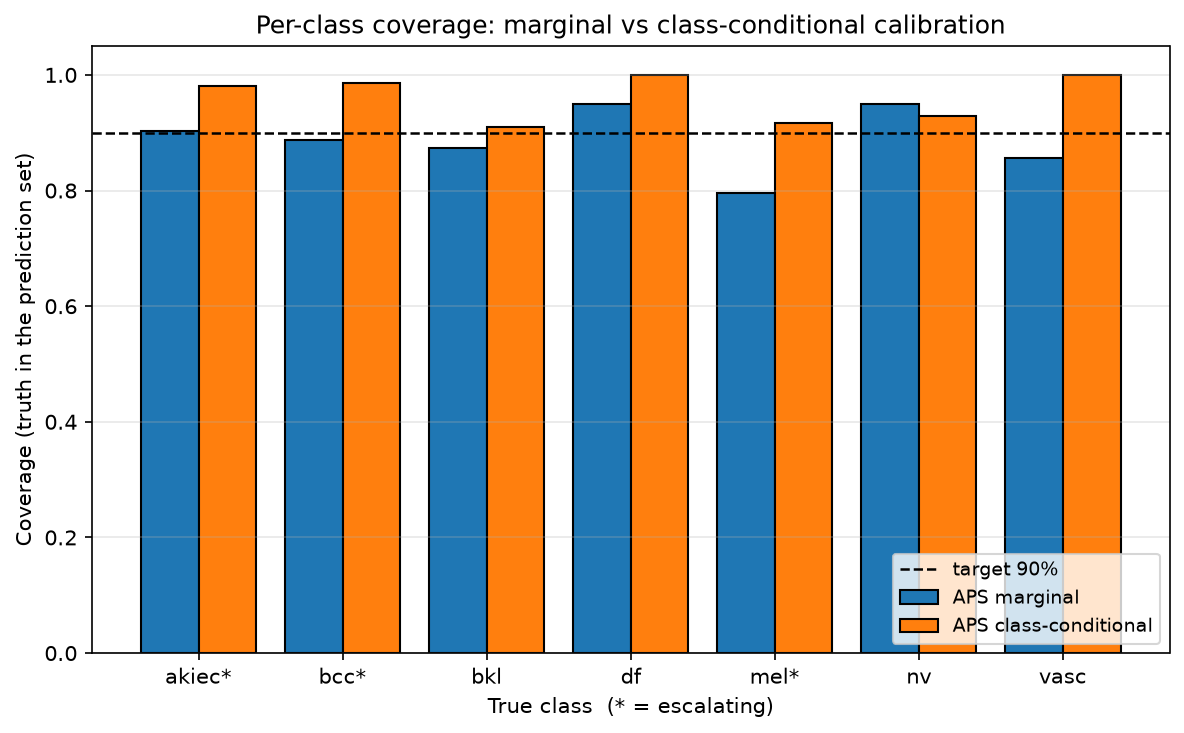
\includegraphics[width=\columnwidth]{figure5_conformal_coverage.png}
\caption{Per-class empirical coverage for APS at $\alpha=0.10$ under marginal and Mondrian
class-conditional calibration, against the $90\%$ target. Marginal calibration (blue) buys
its average from \textsc{nv} and \textsc{df} while under-covering two of the three
escalating classes, worst on \textsc{mel} at $0.796$; \textsc{akiec} lands only just at
target, not below it. Class-conditional calibration (orange) brings every class to or above
target --- raising six of them and trimming \textsc{nv}, which had been over-covered. LAC shows the same pattern more severely (\textsc{mel} $0.671$,
Table~\ref{tab:conformal}).}
\label{fig:conformal}
\end{figure}

\subsection{Subgroup analysis: an age-stratified blind spot}
\label{sec:results-fairness}

Every aggregate number reported so far is consistent with a competent system. Stratifying by
patient age reveals that it is not, uniformly.

% Generated by research/run_session7_stats.py -- do not hand-edit (hard rule 4).
% Test column filled by the S9 single pre-registered test pass.
\begin{table*}[t]
\centering
\caption{Escalation sensitivity by patient age band, with $95\%$ confidence intervals. Intervals marked CP are exact Clopper--Pearson; those marked boot are lesion-grouped percentile bootstrap. The exact interval leads wherever the numerator is small, because the percentile bootstrap cannot reach the upper tail at those counts and would understate the uncertainty. Validation and out-of-fold estimates are shown side by side: the OOF split carries substantially more escalating cases in the under-40 band, which is why the age-conditional rule is fitted there. The test column is reported once, from the single pre-registered pass of Session~9; it is scored by the same deployed system as the OOF column and is not a like-for-like replication of the validation column, which different models scored on different patients.}
\label{tab:agegap}
\begin{tabular}{lcccccc}
\toprule
& \multicolumn{2}{c}{Validation} & \multicolumn{2}{c}{OOF} & \multicolumn{2}{c}{Test} \\
\cmidrule(lr){2-3}\cmidrule(lr){4-5}\cmidrule(lr){6-7}
Age band & Sensitivity [95\% CI] & $k/n$ & Sensitivity [95\% CI] & $k/n$ & Sensitivity [95\% CI] & $k/n$ \\
\midrule
$<$40 & $0.545$ [0.322, 0.756]$^{\text{CP}}$ & $12/22$ & $0.547$ [0.382, 0.716]$^{\text{boot}}$ & $35/64$ & $0.143$ [0.030, 0.363]$^{\text{CP}}$ & $3/21$ \\
40-59 & $0.550$ [0.392, 0.714]$^{\text{boot}}$ & $33/60$ & $0.612$ [0.547, 0.674]$^{\text{boot}}$ & $243/397$ & $0.814$ [0.694, 0.918]$^{\text{boot}}$ & $57/70$ \\
60+ & $0.774$ [0.696, 0.838]$^{\text{boot}}$ & $175/226$ & $0.733$ [0.697, 0.768]$^{\text{boot}}$ & $655/893$ & $0.764$ [0.683, 0.836]$^{\text{boot}}$ & $152/199$ \\
All ages & $0.714$ [0.644, 0.783]$^{\text{boot}}$ & $220/308$ & $0.690$ [0.657, 0.721]$^{\text{boot}}$ & $935/1356$ & $0.731$ [0.665, 0.793]$^{\text{boot}}$ & $212/290$ \\
\bottomrule
\end{tabular}
\par\smallskip\footnotesize Patients with no recorded age are excluded from the bands above: $10$ validation images ($0$ escalating) and $38$ OOF images ($2$ escalating), and $9$ test images ($0$ escalating). They are retained in the All-ages row and in \texttt{age\_gap\_intervals.csv}.
\end{table*}


Table~\ref{tab:agegap} gives escalation sensitivity by age band at full coverage on all three
splits. On test, patients aged $60$ and over have $76.4\%$ of their escalating lesions caught
and the $40$--$59$ band $81.4\%$. Patients under $40$ have $14.3\%$ --- three of twenty-one
--- with eighteen lesions requiring escalation, most of them melanomas, classified as ordinary
nevi. The single pre-specified confirmatory comparison, under $40$ against $60+$ and the sole
member of its family, gives a difference of $-0.621$ $[-0.786, -0.386]$ with Holm-adjusted
$p<0.001$.

\textbf{The gap is established; its magnitude is not, and we report both facts.} The point
estimate $0.143$ rests on twenty-one positives, and its exact interval $[0.030, 0.363]$ is
correspondingly wide --- the percentile bootstrap would have returned $[0.000, 0.286]$ and
understated it. The same quantity is $0.545$ $[0.322, 0.756]$ on validation and $0.547$
$[0.382, 0.716]$ out-of-fold. Those are not a failed replication: they are different splits
scored by different model sets, so they are not like-for-like, and the confirmatory comparison
was pre-specified on out-of-fold data, where it gives $-0.187$ $[-0.370, -0.016]$, Holm
$p=0.036$ --- the same sign and significance at a much smaller magnitude. The $40$--$59$ band
is similarly unstable across splits ($0.550 \rightarrow 0.612 \rightarrow 0.814$). What is
stable across all three splits is the ordering: the under-$40$ band is the worst of the three
every time, and its deficit against $60+$ excludes zero on both splits where it was tested.
The defensible statement is that \emph{a large age gap is established and its magnitude is
not}, and the figure $0.143$ should never be quoted bare.

\textbf{Abstention does not rescue it, and the safety net is thinnest where it is needed most.}
Fig.~\ref{fig:selective}(b) shows a well-behaved aggregate abstention trade-off --- retained-set
metrics improve monotonically with deferral --- which is exactly why the subgroup breakdown is
necessary to see the problem. At a $10\%$ target the gate defers $17.3\%$ of $60+$ cases but
only $6.2\%$ of under-$40$ cases, because confidence is high in that band; the mechanism
recedes precisely where the errors are. Of the misses it then rescues, $36.2\%$ $[0.227,
0.515]$ in the $60+$ band, $15.4\%$ $[0.019, 0.454]$ at $40$--$59$ and $11.1\%$ $[0.014,
0.347]$ under $40$. The two younger bands rest on thirteen and eighteen misses and their
intervals overlap heavily, so we do not claim a resolved ordering between them; the
aggregate carries the claim, and it is stark enough --- across the whole split, only $21$ of
$78$ missed escalating lesions are deferred rather than answered wrongly ($26.9\%$ $[0.175,
0.382]$). The model is not uncertain about these lesions. It is confidently wrong about them,
which places them beyond the reach of any uncertainty-based safety net, including the
conformal machinery of Sec.~\ref{sec:results-conformal} --- as the under-$40$ coverage column
of Table~\ref{tab:bipartite} independently confirms.

\textbf{The mechanism is partly a decision rule and partly lost information, and an earlier
reading of ours was too strong.} A threshold-free diagnostic separates the two possibilities.
Within each band, take the escalating-class probability mass $\sum_{c \in \mathcal{E}} p_c(x)$
and ask how well it ranks truly escalating lesions above benign ones. This uses no threshold,
no prior and no calibration, so it measures what the probability vector \emph{carries}, as
distinct from what the $\arg\max$ rule \emph{does with it}. On validation the answer was
striking: the under-$40$ band separated escalating lesions essentially as well as the older
bands ($0.927$ against $0.933$ and $0.934$), which supports reading the failure as purely a
decision-rule failure --- the signal is there and $\arg\max$ discards it because \textsc{nv}
dominates the band.

That reading weakens as the estimate improves. Out-of-fold, with $64$ escalating under-$40$
cases instead of $22$, the within-band AUC is $0.889$ $[0.831, 0.949]$ against $0.953$ and
$0.934$. On test it is $0.810$, against $0.975$ and $0.933$ in the same two bands on the same
split, where the under-$40$ band also ranks worst rather than comparably. The honest reading
is therefore that the failure is \emph{both}: the probability vector still ranks escalating
lesions under $40$ far above chance, so a decision rule can recover part of the gap, but its
ranking in that band is genuinely weaker, so no threshold recovers all of it. We state this
explicitly because an earlier version of this analysis, built on validation alone, asserted
the pure decision-rule reading. Twenty-one positives is thin, the three estimates disagree,
and the balance between the two mechanisms is not resolved by these data. What the diagnostic
does establish, on every split, is that the signal is not absent --- which is what licenses
attempting a decision-rule mitigation at all.

\textbf{The source is the training prior.} In the training split, $4.9\%$ of lesions in
patients under $40$ require escalation, against $35.5\%$ in the $60+$ band. A model trained to
minimise a class-weighted loss over this distribution learns, correctly with respect to the
training objective and catastrophically with respect to the clinical objective, that a
pigmented lesion on a young patient is a nevus. This is a shortcut in the sense of Geirhos
\emph{et al.}~\cite{geirhos2020shortcut} and an instance of hidden
stratification~\cite{oakdenrayner2020hidden}: a clinically meaningful subpopulation
systematically mishandled while every aggregate metric stays healthy. Melanoma in young adults
is precisely the presentation where early detection carries the largest survival benefit, so
the subgroup with the worst model performance is the subgroup where errors cost the most.

\subsection{An age-conditional decision rule, and what it costs a clinic}
\label{sec:results-utility}

The diagnostic above licenses a mitigation at the decision rule rather than in the model. We
apply the one-parameter rule of Eq.~\eqref{eq:lambda} with the $\lambda_b$ frozen from
out-of-fold fitting, on top of rung A7-oof --- the arm whose calibrated probabilities the
out-of-fold $\lambda$ is dimensionally compatible with --- and read it once on test.
Table~\ref{tab:agerule} reports the result.

\begin{table}[t]
\centering
\caption{The age-conditional escalation rule on the test split, at the $\lambda_b$ frozen from
out-of-fold fitting, against plain $\arg\max$ on the same probabilities (rung A7-oof).
Referral is the share of the band the system escalates. NNB is Number Needed to Biopsy at the
stated reference prevalence $\pi=0.03$ (Eq.~\eqref{eq:nnb}), \emph{not} at this cohort's
prevalence.}
\label{tab:agerule}
\setlength{\tabcolsep}{4pt}
\begin{tabular}{lccccc}
\toprule
Band & $\lambda_b$ & Rule & Sens. [95\% CI] & Referral & NNB$_{0.03}$ \\
\midrule
\multirow{2}{*}{$<40$} & \multirow{2}{*}{$0.26$}
  & $\arg\max$ & 0.143 [0.030, 0.363] & 0.028 & 5.2 \\
  & & $+\lambda$ & 0.238 [0.082, 0.472] & 0.066 & 8.1 \\
\midrule
\multirow{2}{*}{$40$--$59$} & \multirow{2}{*}{$0.74$}
  & $\arg\max$ & 0.814 [0.694, 0.918] & 0.109 & 2.1 \\
  & & $+\lambda$ & 0.971 [0.926, 1.000] & 0.234 & 5.9 \\
\midrule
\multirow{2}{*}{$60+$} & \multirow{2}{*}{$0.33$}
  & $\arg\max$ & 0.764 [0.683, 0.836] & 0.350 & 5.3 \\
  & & $+\lambda$ & 0.844 [0.780, 0.903] & 0.423 & 7.6 \\
\midrule
\multirow{2}{*}{All} & \multirow{2}{*}{---}
  & $\arg\max$ & 0.731 [0.665, 0.793] & 0.178 & 3.0 \\
  & & $+\lambda$ & \textbf{0.831 [0.776, 0.885]} & 0.268 & 6.2 \\
\bottomrule
\end{tabular}
\end{table}

Overall escalation sensitivity rises from $0.731$ to $0.831$ and missed serious cases fall
from $78$ to $49$, at a referral rate rising from $17.8\%$ to $26.8\%$ and a Macro-F1 cost of
$-0.038$ ($0.7871 \rightarrow 0.7492$). The rule helps every band. It helps the $40$--$59$
band most dramatically ($0.814 \rightarrow 0.971$, misses $13 \rightarrow 2$) and the
under-$40$ band least ($0.143 \rightarrow 0.238$) --- exactly the ordering the escalation-mass
diagnostic predicted, since that band has both the largest threshold deficit and the weakest
ranking. Under-$40$ escalation sensitivity remains poor in absolute terms after the
intervention, and we do not present this as a solved problem.

\textbf{Is it redundant with abstention? In two bands no, in the band it was built for, yes.}
Cost-sensitive thresholding was demoted from our ladder because it proved redundant with
margin abstention --- both target low-margin boundary cases. The age rule is aimed at a
different failure, the \emph{confidently} wrong case, so redundancy is not automatic; but it
is a question to be measured rather than asserted. Table~\ref{tab:ortho} intersects the two
mechanisms over the misses each could rescue.

\begin{table}[t]
\centering
\caption{Overlap between the two safety mechanisms on the escalating lesions that plain
$\arg\max$ misses: cases deferred by the abstention gate at a $10\%$ target, and cases the
age-conditional rule reclassifies as escalating. Jaccard is the overlap of the two rescued
sets. A low value means the mechanisms are complementary; $1.00$ means one adds nothing.}
\label{tab:ortho}
\begin{tabular}{lrrrc}
\toprule
Band & Missed & Deferred & Caught by $\lambda$ & Jaccard \\
\midrule
$<40$      & 18 & 2  & 2  & \textbf{1.00} \\
$40$--$59$ & 13 & 2  & 11 & 0.18 \\
$60+$      & 47 & 17 & 16 & 0.83 \\
\midrule
All        & 78 & 21 & 29 & 0.61 \\
\bottomrule
\end{tabular}
\end{table}

In the $40$--$59$ band the two are clearly complementary: abstention reaches two of thirteen
misses and the rule reaches eleven, overlapping on two, for a Jaccard of $0.18$. At $60+$ they
largely coincide ($0.83$). In the under-$40$ band they are \emph{identical}: of eighteen
misses, abstention defers two, the rule catches two, and they are the same two --- Jaccard
$1.00$. This is a negative result inside the paper's own headline contribution and we report
it as measured. In the band the rule was designed for, it is not an independent safety net: it
reaches the same small set of cases the uncertainty gate already reaches, and sixteen
confidently wrong misses are outside both. The counts are small --- eighteen misses --- so the
estimate is unstable, but the direction is unambiguous and it should not be smoothed into the
aggregate figure of $0.61$.

\textbf{What it costs a clinic, with the prevalence assumption stated once.} This paper
carries three instruments that all answer the question ``what would this cost in practice'':
decision curve analysis (Fig.~\ref{fig:dca}), Number Needed to Biopsy
(Table~\ref{tab:agerule}), and the false reassurance rate (Table~\ref{tab:bipartite}). They
share one assumption and we state it here rather than three times. All are computed on a
cohort whose escalating prevalence is $19.3\%$, which is far above the $1$--$5\%$ of
primary-care screening; DCA net benefit and \emph{observed} NNB are therefore internal
comparisons between configurations on this cohort and are not transportable absolute
quantities. Only the re-weighted $\mathrm{NNB}_{\pi}$ of Eq.~\eqref{eq:nnb} is offered as a
clinical figure, and even that assumes the class-conditional score distributions transfer.

Read that way, the age-conditional rule moves overall NNB from $3.0$ to $6.2$ at $\pi=0.03$:
roughly six lesions escalated per escalation-warranting lesion found, against three before,
in exchange for twenty-nine fewer missed serious cases. The sensitivity range is wide ---
$7.1 \rightarrow 16.9$ at $\pi=0.01$ and $2.2 \rightarrow 4.1$ at $\pi=0.05$ --- which is
itself the point: an NNB quoted without its prevalence is not a number a clinician can use.
Whether that trade is acceptable is a question for a care pathway and not for us; what the
analysis provides is the exchange rate, priced in the currency clinicians already use, with the definitions fixed in advance in
Sec.~\ref{sec:metrics}.

\subsection{Three centres: the operating point transfers, the mechanism does not}
\label{sec:results-battery}

% generated by research/external/render_composite_tables.py -- do not hand-edit
% supersedes external_table_{bcn_age_replication,pad_prior_shift,cross_cohort_triage,
%   decision_curve,conformal_shift,fitzpatrick_slices}.tex, which stay on disk as the
%   per-analysis outputs of their own scripts but are no longer part of the manuscript.
\begin{table*}[t]
\centering
\caption{External validity battery. All four panels score the deployed system unmodified -- uniform six-CNN soft-vote, 24-view TTA, frozen HAM10000-OOF Dirichlet map (\texttt{selective/results\_oof/fit\_state.json}) and frozen per-band $\lambda$ ($<$40: $0.26$, 40--59: $0.74$, 60+: $0.33$) -- so no parameter in any row is fitted on the cohort it is evaluated on. Point estimates are image-level; intervals resample lesions, except proportions with fewer than 30 events, which take the exact Clopper--Pearson interval. Panel~(A): the pre-registered contingency fired --- Claim~A (a cohort-invariant escalation-mass AUC) fails, with a spread of 0.105 across centres, and the Claim~B ordering is reversed rather than non-monotonic, so the three point estimates are reported with intervals and no trend is fitted. The confirmatory member \texttt{E1\_under40\_sens\_frozen\_lambda\_vs\_argmax} (BCN-20000, exact McNemar over 27 discordant cases) gives $p = 1.49 \times 10^{-8}$, Holm upper bound over the five-member family $= 7.45 \times 10^{-8}$; because $\lambda \ge 0$ can only add escalating predictions the test is one-sided by construction and certifies that cases were rescued, not that the rule is net-beneficial --- that trade is the last two columns. MSKCC's label space holds only \textsc{nv}, \textsc{mel} and \textsc{bkl}, so seven-class Macro-F1 is undefined there. Panel~(B) confirmatory member \texttt{E2\_em\_macro\_f1\_vs\_raw} is significant in the \emph{wrong} direction ($\chi^2 = 98.73$, $p = 2.89 \times 10^{-23}$, 321 cases correct only without the correction against 113 only with it). Panel~(C) point-FRR is the fraction of malignant Tier-1 lesions predicted Tier~3; NNB is the number needed to biopsy at reference prevalence $\pi$. $^{\dagger}$Panel~(D)'s test column is reconstructed from the frozen Session~9 artifacts (\texttt{results/session9/agerule\_test.csv}: TP, FP and $N$ only) and involves no new read of the test split.}
\label{tab:external_battery}
\scriptsize
\setlength{\tabcolsep}{3.2pt}
\begin{tabular}{@{}lcccccccc@{}}
\toprule
\multicolumn{9}{@{}l}{\textbf{(A) Three-centre dose--response of the under-40 escalation failure (E1).} Centres ordered by ascending prior skew. No parameter is fitted on BCN-20000 or MSKCC.} \\
\addlinespace[0.2em]
Cohort & Skew & \multicolumn{3}{c}{Escalation-mass AUC by age band} & \multicolumn{4}{c}{Under-40 escalation sensitivity} \\
\cmidrule(lr){3-5}\cmidrule(l{0.4em}){6-9}
 & $60{+}/{<}40$ & $<$40 [95\% CI] & 40--59 & 60+ & argmax [95\% CI] & mel.\ only & frozen $\lambda$ & $\Delta$ referral \\
\midrule
BCN-20000 & 3.83$\times$ & 0.791 [0.726, 0.843] & 0.826 & 0.795 & 0.279 [0.179, 0.382] & 0.274 & \textbf{0.352} & +0.026 \\
MSKCC & 6.54$\times$ & 0.790 [0.703, 0.867] & 0.693 & 0.694 & 0.333 [0.186, 0.510] & 0.333 & \textbf{0.389} & +0.019 \\
HAM10000 (source) & 8.45$\times$ & 0.895 [0.837, 0.944] & 0.955 & 0.934 & 0.547 [0.391, 0.708] & 0.490 & \textbf{0.625} & +0.024 \\
\midrule
\multicolumn{9}{@{}l}{\textbf{(B) PAD-UFES-20 prior decoupling (E2).} All $N=2{,}106$ images, no weights retrained. \textsc{oracle} uses the true target prior and is a ceiling, not a deployable system.} \\
\addlinespace[0.2em]
Variant & Deployable & Macro-F1 & Bal.\ acc. & Accuracy & Esc.\ sens. & Mel.\ recall & Missed serious &  \\
\midrule
Raw soft-vote & yes & 0.1669 & 0.3097 & 0.2626 & 0.3565 & 0.1154 & 1{,}047 &  \\
Dirichlet (deployed) & yes & 0.1303 & 0.2931 & 0.2137 & 0.2207 & 0.1154 & 1{,}268 &  \\
EM prior (Saerens) & yes & 0.1018 & 0.1035 & 0.1638 & 0.4155 & 0.0000 & 951 &  \\
Oracle prior & \textsc{oracle} & 0.2534 & 0.3327 & 0.4435 & 0.8949 & 0.0577 & 171 &  \\
Dirichlet $\rightarrow$ EM & yes & 0.1239 & 0.3079 & 0.2203 & 0.1223 & 0.0000 & 1{,}428 &  \\
\midrule
\multicolumn{9}{@{}l}{\textbf{(C) Three-tier clinical actionability (E3).} Tier~1 urgent biopsy (\textsc{mel}, \textsc{bcc}, \textsc{scc}); Tier~2 consult (\textsc{akiec}); Tier~3 discharge.} \\
\addlinespace[0.2em]
Cohort / configuration & Tier acc. & T1 sens. & T1 spec. & point-FRR & Missed T1 & \multicolumn{3}{c}{NNB at $\pi = 0.01/0.03/0.05$} \\
\cmidrule(l{0.4em}){7-9}
\midrule
HAM10000 OOF, raw & 0.8936 & 0.6781 & 0.9509 & 0.2875 & 326 & 8.17 & 3.34 & 2.38 \\
HAM10000 OOF, calibrated & 0.8986 & 0.6578 & 0.9584 & 0.3289 & 373 & 7.25 & 3.04 & 2.20 \\
PAD-UFES-20, raw & 0.3732 & 0.2698 & 0.9446 & 0.5195 & 466 & 21.34 & 7.64 & 4.90 \\
PAD-UFES-20, calibrated & 0.3310 & 0.2185 & 0.9644 & 0.6756 & 606 & 17.11 & 6.26 & 4.09 \\
PAD-UFES-20, oracle prior & 0.4720 & 0.4771 & 0.7469 & 0.0524 & 47 & 53.51 & 18.15 & 11.08 \\
\midrule
\multicolumn{9}{@{}l}{\textbf{(D) Decision-curve net benefit of the frozen age rule (E6).} $\mathrm{NB} = \mathrm{TP}/N - (\mathrm{FP}/N)\,p_t/(1-p_t)$; $\Delta$ is $\lambda$-rule minus argmax under a lesion-grouped paired bootstrap, bold where the interval excludes zero.} \\
\addlinespace[0.2em]
$p_t$ & Biopsy all & Argmax & $\lambda$-rule & Risk model & $\Delta$ & 95\% CI & Test $\Delta^{\dagger}$ &  \\
\midrule
\multicolumn{9}{@{}l}{\textit{All ages}} \\
0.05 & 0.1518 & 0.1327 & 0.1589 & 0.1759 & \textbf{+0.0263} & [+0.0214, +0.0315] & +0.0156 &  \\
0.10 & 0.1047 & 0.1306 & 0.1534 & 0.1633 & \textbf{+0.0228} & [+0.0178, +0.0282] & +0.0114 &  \\
0.15 & 0.0520 & 0.1283 & 0.1472 & 0.1544 & \textbf{+0.0189} & [+0.0138, +0.0243] & +0.0067 &  \\
0.20 & -0.0072 & 0.1257 & 0.1403 & 0.1449 & \textbf{+0.0146} & [+0.0093, +0.0199] & +0.0015 &  \\
\multicolumn{9}{@{}l}{\textit{Age $<$40}} \\
0.05 & -0.0016 & 0.0253 & 0.0280 & 0.0280 & +0.0027 & [-0.0002, +0.0065] & +0.0053 &  \\
0.10 & -0.0572 & 0.0239 & 0.0254 & 0.0195 & +0.0015 & [-0.0015, +0.0053] & +0.0034 &  \\
0.15 & -0.1194 & 0.0224 & 0.0226 & 0.0144 & +0.0002 & [-0.0032, +0.0042] & +0.0014 &  \\
0.20 & -0.1893 & 0.0207 & 0.0193 & 0.0125 & -0.0013 & [-0.0053, +0.0029] & -0.0009 &  \\
\bottomrule
\end{tabular}
\end{table*}


\begin{figure*}[t]
\centering
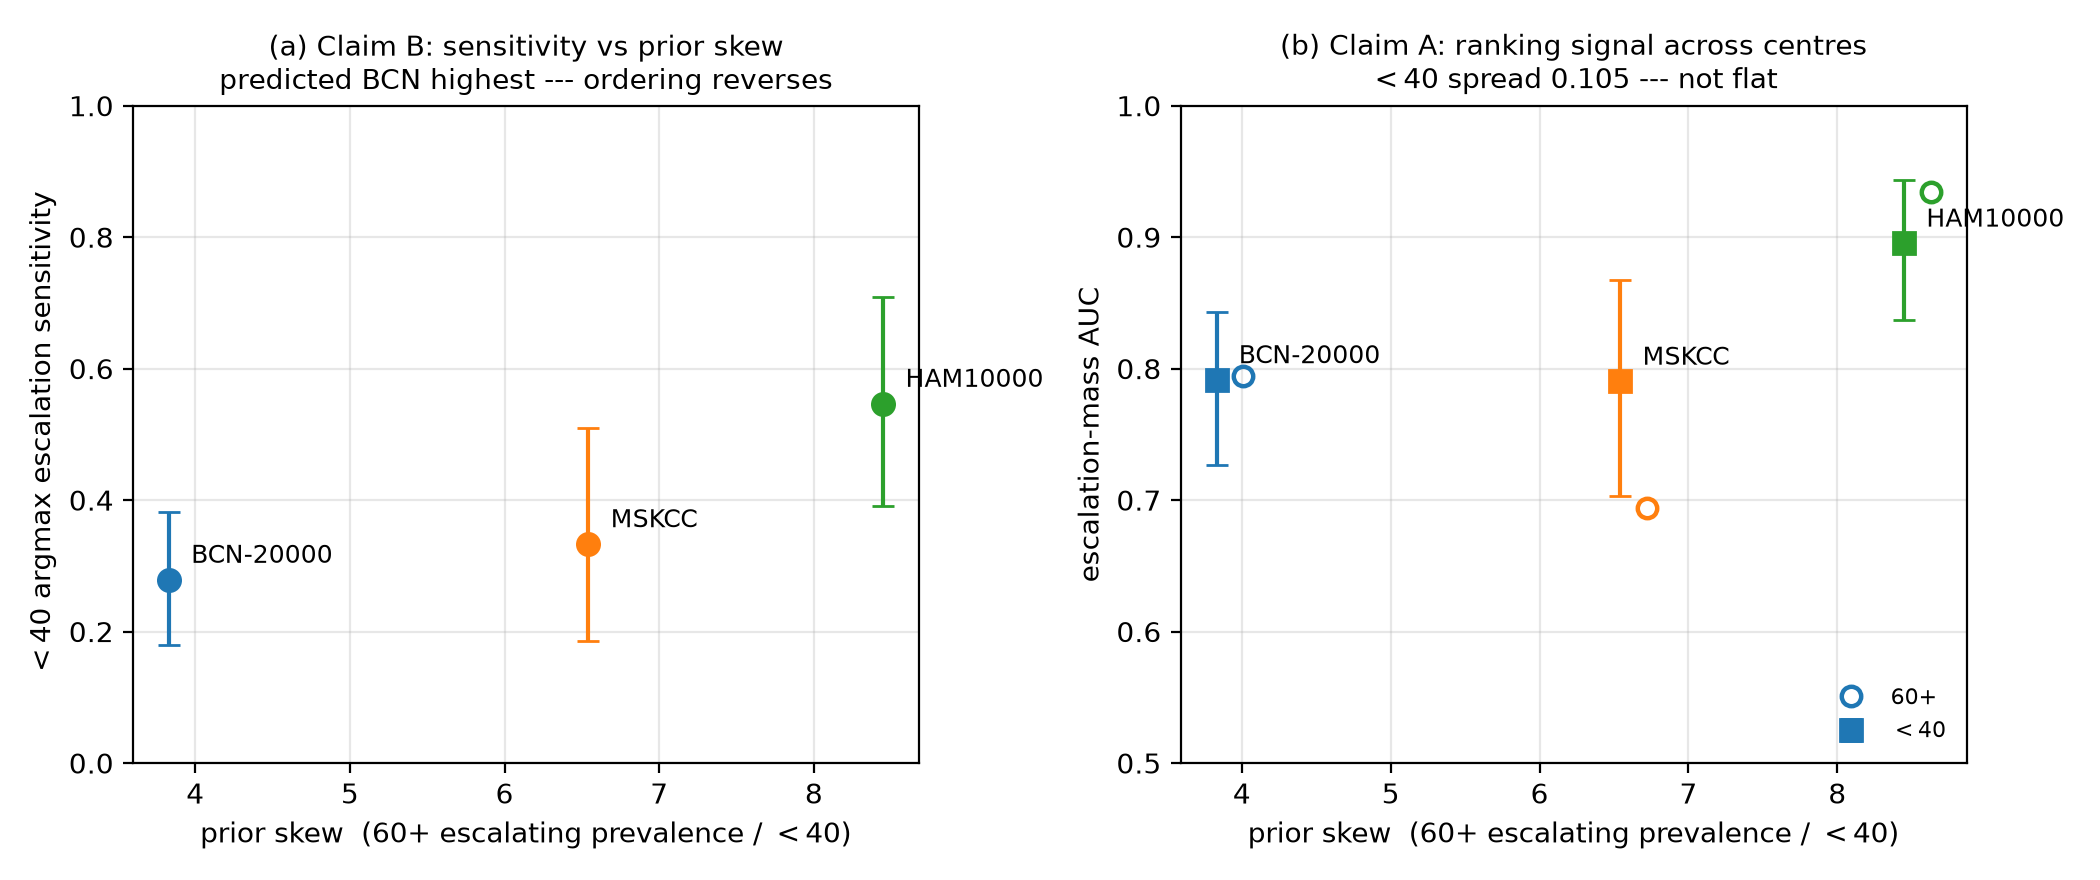
\includegraphics[width=0.82\textwidth]{external_figure_dose_response.png}
\caption{The pre-registered dose--response test, and its outcome. \textbf{(a)} Claim~B
predicted that under-$40$ escalation sensitivity would fall as the training prior's age skew
rises, so that BCN-20000 --- the least skewed centre --- would score highest. The observed
ordering is the exact reverse, and the HAM10000 and BCN-20000 intervals do not overlap.
\textbf{(b)} Claim~A predicted a cohort-invariant escalation-mass AUC; the under-$40$ spread
across centres is $0.105$, and within MSKCC the under-$40$ band is the \emph{best}-ranked
band rather than the worst. Error bars are lesion-grouped bootstrap intervals on the
under-$40$ band, the pre-registered quantity; the $60+$ points are plotted as point estimates
for reference and carry none. Both pre-registered
claims fail, and the contingency declared before the data were seen was to report the three
estimates with intervals, drop the trend language, and offer no post-hoc explanation.}
\label{fig:dose_response}
\end{figure*}

The PAD-UFES-20 result of Sec.~\ref{sec:results-external} is a modality change, and a
modality change confounds everything at once. Workstream~E1 therefore asks the narrower
question the under-$40$ finding actually needs: does the failure reproduce in
\emph{dermoscopy} acquired somewhere else? We score two further ISIC-2019
centres~\cite{combalia2019bcn20000, codella2018isic} with the identical frozen system ---
BCN-20000 ($11{,}982$ images after the pre-registered \textsc{scc} exclusion) and MSKCC
($2{,}903$) --- fitting nothing on either. Two claims were registered in advance. Claim~A: if
the under-$40$ deficit is a decision-rule artefact rather than lost ranking signal,
escalation-mass AUC should be roughly cohort-invariant. Claim~B: if the training prior's age
skew is the cause, under-$40$ sensitivity should track that skew, so the least skewed centre
should do best. Table~\ref{tab:external_battery}, panel~A, and Fig.~\ref{fig:dose_response}
report both.

\textbf{Both claims fail, and Claim~B fails backwards.} The under-$40$ escalation-mass AUC is
$0.895$ $[0.837, 0.944]$ on HAM10000, $0.791$ $[0.726, 0.843]$ on BCN-20000 and $0.790$
$[0.703, 0.867]$ on MSKCC --- a spread of $0.105$, which is not invariance. The
\emph{within}-cohort statement fails too: under-$40$ is the worst-ranked band on HAM10000 and
essentially tied on BCN-20000 ($0.791$ against $0.795$ at $60+$), but on MSKCC it is the
\emph{best}-ranked band ($0.790$ against $0.694$). Claim~B predicted
BCN-20000 $>$ MSKCC $\approx$ HAM10000 in under-$40$ sensitivity; the observed order is
HAM10000 $0.547$ $>$ MSKCC $0.333$ $>$ BCN-20000 $0.279$, the exact reverse, and the
HAM10000 and BCN-20000 intervals do not overlap. Two robustness checks, both declared before
they were computed, leave the reversal intact: restricting to melanoma removes any effect of
differing escalating-class mixes and gives $0.490$ / $0.333$ / $0.274$, and moving from
images to lesions gives $0.500$ / $0.333$ / $0.211$, widening it. The pre-registered
contingency for this outcome was to report the three point estimates with intervals, drop the
trend language, and offer no post-hoc explanation, and that is what we do.

\textbf{One design limitation, recorded as a limitation.} The dose variable is entangled with
transfer quality: BCN-20000 has the lowest skew \emph{and} is the centre the frozen system
transfers to worst, with an all-ages Macro-F1 of $0.402$ against HAM10000's $0.784$. Its
under-$40$ sensitivity is therefore not a clean read of the skew mechanism, and the experiment
is better described as non-decisive than as evidence against the mechanism. We record this
because it is true of the design, not as grounds to retain the hypothesis: a test that could
only have confirmed is not a test, and the contingency above was fixed in advance precisely
so that this paragraph could not become a rescue.

\textbf{What does transfer is the operating point.} The frozen per-band $\lambda$, carried
across unmodified with no target tuning, raises under-$40$ escalation sensitivity in all three
centres: $0.547 \rightarrow 0.625$ on HAM10000, $0.279 \rightarrow 0.352$ on BCN-20000,
$0.333 \rightarrow 0.389$ on MSKCC, at referral-rate costs of $+0.024$, $+0.026$ and $+0.019$.
This is the first same-modality evidence for the intervention; the PAD probe of
Sec.~\ref{sec:results-external} had an inverted class prior and could not supply it. The
pre-registered confirmatory member is an exact McNemar test of the rule against argmax in
BCN-20000's under-$40$ band, and it is significant ($p = 1.49\times10^{-8}$, Holm upper bound
$7.45\times10^{-8}$ over the five-member external family). We deliberately do not lean on that
$p$-value. Because $\lambda \ge 0$ can only move a prediction \emph{towards} the escalating
classes, no case caught by argmax can be lost by the rule, the discordant cell in one
direction is structurally zero, and the test reduces to asking whether any case was rescued at
all. It certifies that $27$ were. Whether that is worth $2.6$ additional referrals per hundred
is a question the trade in panel~A answers and the $p$-value cannot. A target-fitted sweep,
reported as descriptive only, puts the under-$40$ optimum at $\lambda = 0.24$ on HAM10000
against the frozen $0.26$ --- a reassuring sanity check --- but at $0.12$ on MSKCC and $0.91$
on BCN-20000, which is the honest version of the same point: the direction exports, the exact
threshold does not.

\begin{figure*}[t]
\centering
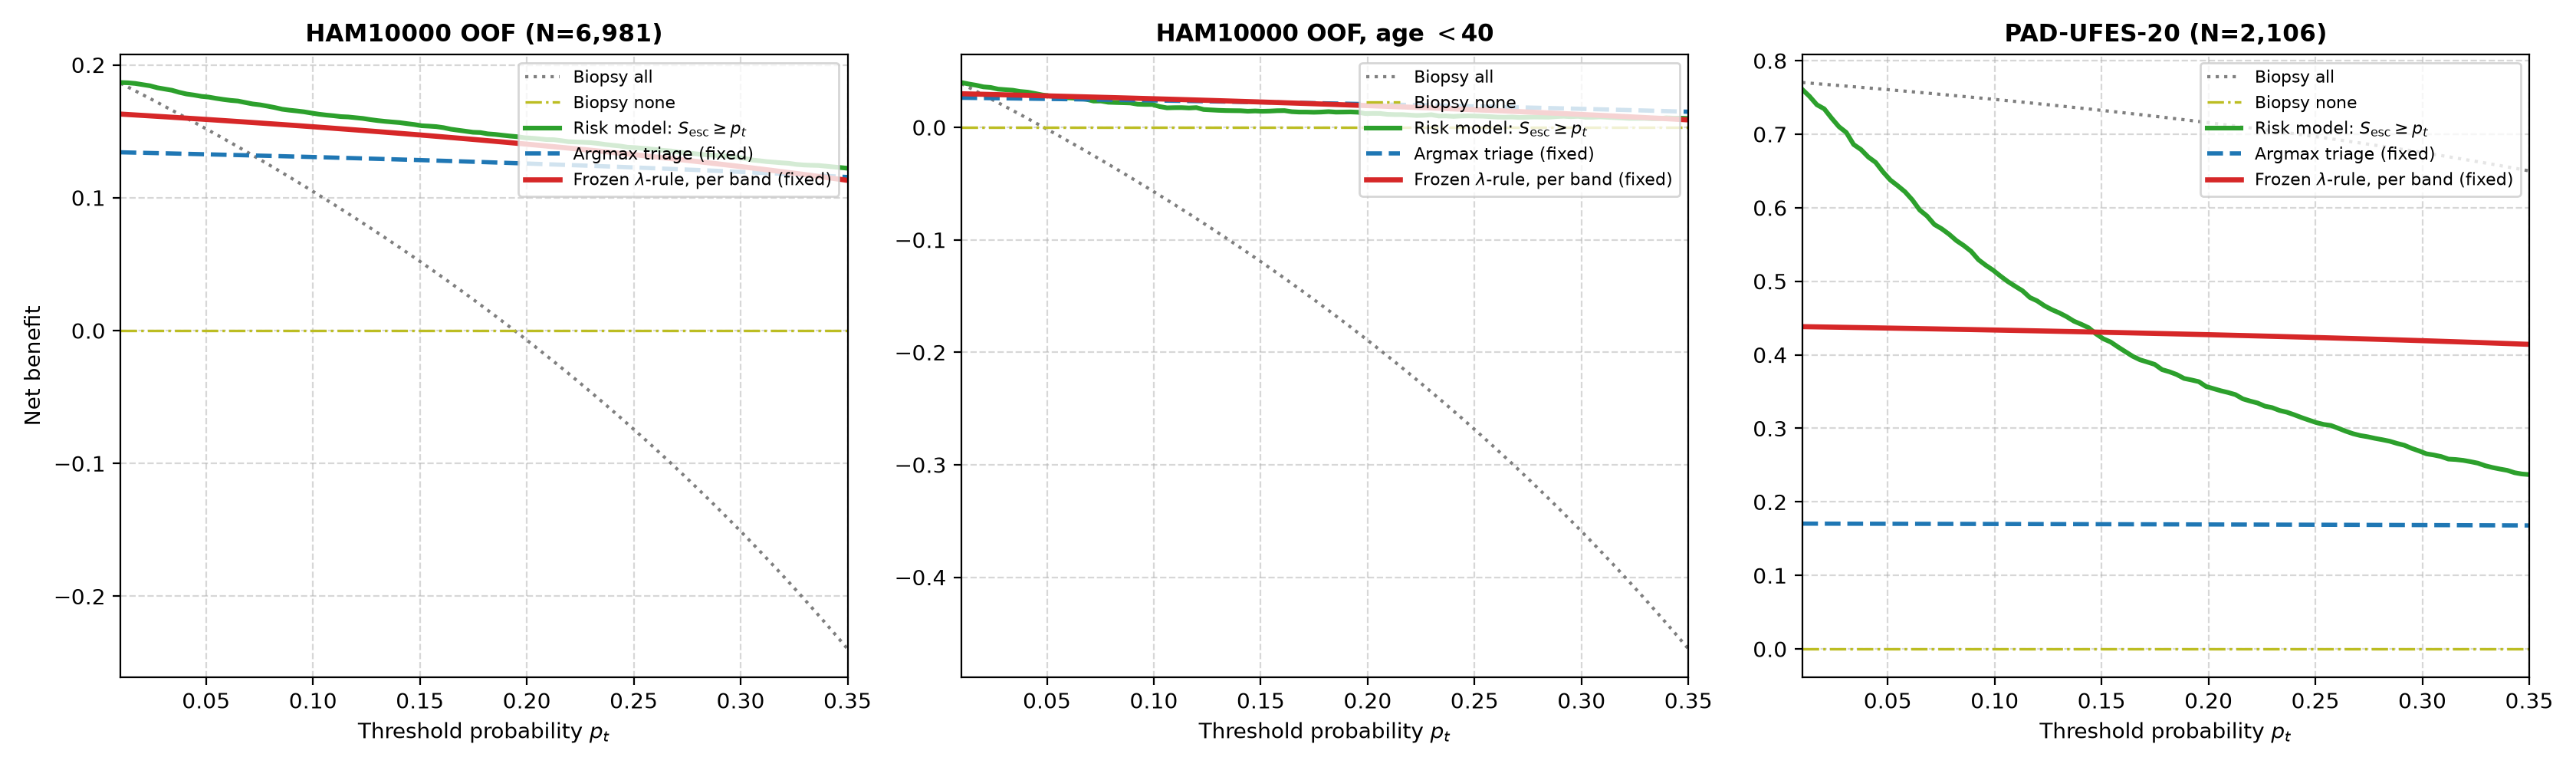
\includegraphics[width=0.94\textwidth]{external_figure_decision_curve.png}
\caption{Decision curves for the frozen age-conditional rule. Net benefit against threshold
probability $p_t$ for biopsy-all, biopsy-none, argmax triage, the frozen $\lambda$-rule, and a
risk model that thresholds the escalation mass $S_{\mathrm{esc}}$ directly. The $\lambda$-rule
and argmax are fixed operating points: they refer the same cases at every $p_t$, so their true-
and false-positive counts do not vary, but their net benefit still declines in $p_t$ because the
false-positive term carries the odds weight $p_t/(1-p_t)$. Only the risk model changes
\emph{which} cases it refers as $p_t$ moves, which is why its curve is the steeper one. \textbf{Left}: the full out-of-fold panel, where the rule dominates argmax
across the plausible range. \textbf{Centre}: the under-$40$ band alone, where the two are
indistinguishable and the ordering inverts by $p_t = 0.20$. \textbf{Right}: PAD-UFES-20, where
the inverted prior lifts every strategy's net benefit and the comparison says little about the
rule. Paired intervals are in Table~\ref{tab:external_battery}, panel~D.}
\label{fig:dca}
\end{figure*}

\textbf{The rule earns its referrals overall, and does not earn them where it was aimed.}
Panel~D of Table~\ref{tab:external_battery} and Fig.~\ref{fig:dca} give the decision-curve
comparison, with lesion-grouped paired bootstrap intervals on the difference. Across all ages
the $\lambda$-rule beats argmax triage at every threshold probability we examined, by
$+0.0228$ $[+0.0178, +0.0282]$ in net benefit at $p_t = 0.10$. Within the under-$40$ band the
same difference is null at every threshold ($+0.0015$ $[-0.0015, +0.0053]$ at $p_t = 0.10$)
and turns negative by $p_t = 0.20$. The test column, reconstructed from the frozen Session~9
artifacts without a new read of the test split, agrees in sign and magnitude throughout. This
is the same shape as the internal result of Sec.~\ref{sec:results-utility}: the rule helps
every band and helps the under-$40$ band least, which is what one expects if part of that
band's deficit is lost ranking signal that no threshold can recover.

\textbf{Read as a clinical action, the numbers are sobering.} Panel~C of
Table~\ref{tab:external_battery} collapses the seven classes into three tiers --- urgent
biopsy, consultation, discharge --- and reports the number needed to biopsy at reference
prevalences. In distribution the system needs $3.0$ biopsies per malignancy found at
$\pi = 0.03$ and sends $373$ of $6{,}981$ Tier-1 lesions to discharge; on PAD-UFES-20 the same
configuration needs $6.3$ and its point-wise false-reassurance rate is $0.676$. The distance
between those two columns is the entire content of the deployability claim in this paper.


\textit{The ablation ladder, the five negative combination levers, selective classification, explainability, the intersectional slices and the smartphone clinical-photography evaluation are reported in full in Appendix~\ref{app:extresults}.}
% =====================================================================
\section{Discussion}

\subsection{Marginal guarantees are the wrong guarantee --- and class-conditional ones are
not automatically the right one}
The conformal result generalises beyond this dataset. Any screening problem with a dominant
benign class will allow a marginal coverage guarantee to be satisfied almost entirely by the
majority, and the more imbalanced the problem, the more comprehensively the guarantee can be
satisfied while failing the patients it exists to protect. Our $\alpha=0.10$ LAC configuration
is formally valid, empirically on-target at $90.1\%$, and leaves roughly one malignant lesion
in four with a shortlist containing nothing that would prompt referral.

The sharper point is the one we did not anticipate. Repairing this by conditioning on the
\emph{label} --- Mondrian class-conditional calibration --- restores aggregate malignant
coverage to about $0.89$--$0.90$ and still leaves malignant lesions in patients under $40$
covered at $0.57$--$0.67$. Label-conditional validity is blind to patient-level structure.
Conditioning jointly on the patient's age band and the escalation requirement, an instance of
equalised coverage~\cite{romano2020equalized}, raises that to $0.86$--$0.95$ at no cost in set
size, because six well-populated cells estimate their quantiles more sharply than seven cells
two of which are nearly empty. We would suggest that medical applications of conformal
prediction report coverage conditioned on the clinically positive set \emph{and} on the
subgroups the system is meant to serve, and that marginal coverage alone be treated as
insufficient evidence of validity. The natural endpoint for such reporting is a quantity like
the false reassurance rate of Eq.~\eqref{eq:frr}, stated with an interval, together with the
$\alpha$ required to bound it rather than a bound chosen in advance.

\subsection{Confidently wrong is a distinct failure mode --- and the mechanism is in the
summary, not only in the model}
The selective-classification literature is largely built on the premise that a model's
uncertainty correlates with its errors, and our aggregate risk--coverage curves support that
premise. The age analysis shows where it breaks: in the under-$40$ band the model's errors are
not accompanied by elevated uncertainty, and the abstention gate defers a \emph{smaller}
fraction of that band ($6.2\%$) than of the $60+$ band ($17.3\%$), so the safety net thins out
exactly where it is needed.

An earlier version of this work drew a strong conclusion from that: that no abstention rule,
conformal set or calibration map built from the same probability vector could detect an error
the probability vector does not signal. That claim was too strong and we correct it. The
probability vector \emph{does} carry signal here. Within the under-$40$ band, escalating-class
mass ranks truly escalating lesions above benign ones at AUC $0.810$ on test, $0.889$
out-of-fold and $0.927$ on validation. What fails is the \emph{summary} each safety mechanism
takes of that vector: abstention reads the top-two margin or the maximum probability, both
large whenever $p(\textsc{nv})$ is large; conformal set construction inherits the same
ordering; and a global calibration map applies one function identically to every patient. Each
discards the escalating-mass direction, which is where the residual signal lives. That is a
correctable defect of the summaries, and our one-parameter rule --- which reads exactly that
direction --- recovers part of the gap ($0.143 \rightarrow 0.238$) where abstention recovers
almost none.

Only part, though, and we are careful about the remainder. The within-band AUC is also
genuinely lower under $40$ than in the older bands on the test split, so some of the gap is
lost ranking ability that no decision rule reading this probability vector can recover; the
three splits disagree about how much. And in that same band the rule turns out to rescue
exactly the two cases abstention already rescued (Table~\ref{tab:ortho}), so the two
mechanisms are not independent there --- a negative result inside our own contribution. The
defensible statement is that the failure is part decision rule and part information, that the
decision-rule part is addressable and worth addressing, and that the information part is not,
by post-hoc means, on this data.

\subsection{Hidden stratification, and the delta we claim over it}
None of this is a new species of problem. Oakden-Rayner
\emph{et al.}~\cite{oakdenrayner2020hidden} named hidden stratification and showed that
clinically meaningful subclasses routinely fail while aggregate metrics stay healthy;
Seyyed-Kalantari \emph{et al.}~\cite{seyyedkalantari2021underdiagnosis} demonstrated the same
for underdiagnosis across patient groups in chest radiography. Our finding sits squarely in
that lineage, and the training prior we identify makes it a shortcut in the sense of Geirhos
\emph{et al.}~\cite{geirhos2020shortcut}, with the same structure as the site confound of Zech
\emph{et al.}~\cite{zech2018confounding}.

What we would claim to add is three things that prior work did not measure. First, the
mechanism: a threshold-free within-band statistic that separates ``the representation cannot
see it'' from ``the decision rule throws it away'', with the finding that on these data it is
both. Second, that the \emph{safety mechanisms} --- abstention, calibration, conformal
coverage --- are themselves inoperative in the affected subgroup, which is a stronger and more
actionable statement than that the classifier is worse there; an aggregate risk--coverage
curve or reliability diagram can look excellent while the mechanism it describes is switched
off for the population that needs it. Third, a mitigation with a priced clinical cost:
a group-specific threshold in the sense of Hardt \emph{et al.}~\cite{hardt2016equality},
reported not as an accuracy delta but in Number Needed to Biopsy at a stated reference
prevalence, which is the currency in which the trade is actually made.

\subsection{What exports is the intervention, not the explanation}
Carrying the frozen system to three further cohorts separates two things that a
single-dataset paper cannot tell apart: whether the \emph{finding} generalises, and whether
the \emph{fix} does. The answer is uncomfortable and, we think, more useful than a clean
transfer would have been. The fix generalises. A per-band $\lambda$ fitted once on
HAM10000 out-of-fold data raises under-$40$ escalation sensitivity in two independent
dermoscopic centres and in a smartphone cohort with an inverted class prior, at a referral
cost of two to three cases per hundred, with nothing re-fitted anywhere. The explanation does
not. Neither pre-registered claim survived: escalation-mass AUC is not cohort-invariant
(spread $0.105$), and under-$40$ sensitivity did not track the training prior's age skew ---
it tracked it in reverse.

The honest reading is that we have a transportable \emph{operating point} and a
non-transportable \emph{mechanism}, and that this is the normal state of affairs for
threshold-based mitigations rather than a peculiarity of our data. A group-conditional
threshold encodes a policy --- escalate more readily in a group where the base rate misleads
the argmax --- and policies survive a change of cohort in a way that causal stories about why
the base rate misleads do not. The corollary for deployment is concrete and cuts against how
such rules are usually shipped: the \emph{direction} of the correction can be
imported, but its magnitude cannot. A target-fitted sweep puts the under-$40$ optimum at
$\lambda = 0.12$ in one external centre and $0.91$ in the other, against $0.26$ frozen from
the source. A site adopting this system should therefore inherit the rule's form and re-fit
its scalar on local data, which needs a few dozen labelled escalating cases in the affected
band rather than a retraining corpus. That is a much weaker requirement than local
retraining, and a much stronger one than "it worked in the paper".

The same asymmetry appears one level down, in the safety nets. Mahalanobis distance --- worst
of seven scores in distribution --- separates in-distribution from shifted data at AUROC
$0.913$, and the conformal sets widen when it fires, which is the behaviour one wants. But
serious-class coverage still falls from $0.950$ to $0.591$ under that shift, because split
conformal's guarantee is a statement about exchangeability and exchangeability is precisely
what a new imaging modality destroys. A widening set is a warning that the guarantee has
lapsed, not a replacement for it. Systems of this kind should be shipped with the shift
detector wired to a refusal, not to a wider shortlist.

\subsection{Clinical positioning}
We do not claim this system is deployable. The configuration we would put forward for
prospective evaluation is the TTA ensemble with Dirichlet calibration; the age-conditional
escalation rule of Eq.~\eqref{eq:lambda} to restore screening sensitivity; a probability-based
abstention gate at roughly $10\%$ deferral, understood as a second and partly overlapping net
rather than an independent one; and RAPS conformal sets under bipartite calibration as the
output format --- a shortlist, not a diagnosis. On our test split that configuration catches
$83.1\%$ of escalating lesions and issues a reassuring shortlist for $1.4\%$ $[0.4\%, 3.5\%]$
of malignant lesions at $\alpha=0.05$.

Two caveats belong with that recommendation rather than in a separate section. Even after
mitigation, under-$40$ escalation sensitivity is $0.238$, and we would not deploy this system
to that population; the analysis identifies a problem and prices a partial remedy, it does not
solve it. And the entire evaluation is retrospective, on a curated cohort whose escalating
prevalence is four to twenty times that of primary-care screening, so every absolute utility
figure here is an internal comparison rather than a clinical forecast.


\textit{A subsection on which components actually moved the needle appears in Appendix~\ref{app:extdiscussion}.}
% =====================================================================
\section{Limitations}
\label{sec:limitations}

\textbf{Data: one training cohort, three external ones, and a population none of them
covers.} All training is on HAM10000. Applied unmodified to PAD-UFES-20 smartphone
photographs, the six-CNN ensemble reaches Macro-F1 $0.167$ --- below its own best member
($0.188$) --- and the frozen calibration map degrades it further to $0.130$
(Sec.~\ref{sec:results-external}); ensembling, the one rung that clears significance
in-distribution, is the component that transfers worst, because member errors become
correlated under shift. Nothing here licenses pointing a dermoscopy-trained classifier at
phone photographs, and that evaluation is a shift benchmark, not a second validation. The two
dermoscopic centres are a genuine same-modality external test but carry their own limits:
MSKCC's label space holds three of our seven classes, so seven-class Macro-F1 is undefined
there, and BCN-20000 is the centre the frozen system transfers to worst
(Sec.~\ref{sec:results-battery}). On skin tone, HAM10000 has no Fitzpatrick labels and an
individual typology angle proxy computed from image statistics is invalid on dermoscopy ---
vignetting and erythema dominate the measured angle --- so we report none; the external cohort
supplies real labels for types I--IV, where the sensitivity spread is $0.102$ and
non-monotonic, while types V and VI are represented by nine images in total and are
suppressed. This work therefore has nothing to say about darker skin, the population where
published disparities are largest~\cite{daneshjou2022disparities}, and answering that
question requires a corpus that contains it~\cite{groh2021fitzpatrick17k}.

\textbf{Protocol: the out-of-fold move closes one problem and opens two, and one test read
means one test read.} The validation split no longer does six jobs: calibration, thresholds,
abstention quantiles and conformal quantiles are fitted on $6{,}981$ out-of-fold rows, which
quintuples the rarest class's calibration support and eliminates every degenerate conformal
cell at $\alpha=0.05$. It costs something on both sides. Out-of-fold calibration is fitted by
models trained on $80\%$ of the data and applied to a model trained on all of it, a stacking
mismatch we measure but cannot remove, and rung A7-oof is $0.018$ Macro-F1 below its
validation-fitted counterpart. Out-of-fold conformal calibration forfeits the exact
finite-sample guarantee, because calibration and test scores no longer come from one fixed
score function; we audit its coverage empirically and never assert it. Cross-conformal or CV+
would restore a $(1-2\alpha)$ guarantee but requires scoring the test split with all five fold
models, a second test read our protocol does not permit. Relatedly, rung A8 reuses the
six-member out-of-fold Dirichlet map rather than one fitted for a $30$-member vote, and a
$30$-member vote is more hedged than a six-member one, so its negative result is a lower
bound on fold-bagging rather than a refutation of it --- a caveat pre-registered rather than
added once the number came back. Every test quantity in this paper was named before it was
computed, and any analysis these numbers suggest cannot be run against this test split at
all; that is the intended cost of the discipline.

\textbf{The mitigation: right form, locally wrong magnitude, and not orthogonal where it
matters.} Each $\lambda_b$ minimises expected cost under our cost matrix subject to a
per-band specificity floor. The principled objective for a group-specific threshold is
equality of opportunity~\cite{hardt2016equality} --- equal true-positive rates across bands
--- the same computation under a different criterion, and the cleaner choice; we did not make
it, and our under-$40$ $\lambda$ has a bootstrap interval touching zero, so that band's
parameter is the least certain of the three. The external centres sharpen the point: the
frozen value helps everywhere, but a target-fitted sweep puts the under-$40$ optimum at
$0.12$ and $0.91$ in the two external cohorts against $0.26$ frozen from the source, so a
site adopting this rule should inherit its form and re-fit its scalar locally. The
dose--response test that would have explained \emph{why} the rule is needed is non-decisive
by construction, because the cohort with the least prior skew is also the cohort the system
transfers to worst, and we report that as a limitation of the design rather than as a reason
to retain the hypothesis. Finally, the two safety mechanisms are not independent where it
counts: at the $10\%$ operating point the age rule and the abstention gate rescue the same two
of eighteen under-$40$ misses (Table~\ref{tab:ortho}), they are complementary at $40$--$59$
and largely redundant at $60+$, and sixteen confidently wrong under-$40$ misses are reached by
neither. We have no proposal that reaches them. The intersectional slice
(Sec.~\ref{sec:results-intersectional}) narrows the affected population further than our power
gates allow us to characterise: the under-$40$ male cell misses the reporting floor by a
single escalating case.

\textbf{Evidence quality: two attributions corrected, one component not built.} An earlier
version of this work attributed the width of the Macro-F1 intervals and the ladder's
unresolvability to \textsc{df} and \textsc{vasc} scarcity. That conflates two things. The
\emph{level} of Macro-F1 is dragged down by \textsc{akiec} ($F_1 = 0.697$) and \textsc{mel}
($0.699$) --- the two lowest per-class scores on test, one of them the clinically decisive
class --- and not by \textsc{df} ($0.791$) or \textsc{vasc} ($0.842$). The \emph{variance} is
dominated by \textsc{df} and \textsc{vasc}, whose intervals are $0.389$ and $0.308$ wide on
$20$ and $21$ images. Rare-class scarcity widens the intervals; melanoma performance holds the
point estimate down. Separately, the lesion-interior attribution fraction over all $1{,}502$
test images ($0.523$, concentration ratio $3.45$) replaces an earlier $28$-image frame
heuristic, but is computed with respect to the predicted class, so misclassified images score
higher than correct ones; it supports a qualitative claim about where the network looks and
nothing stronger (Sec.~\ref{sec:results-gradcam}), and the mechanistic argument is carried by
the escalation-mass AUC instead. A Shades-of-Grey colour-constancy step was planned and not
implemented; we report its absence rather than leaving an empty row in the ablation.

\textbf{Age is a proxy for something we do not observe.} We stratify by recorded patient age
because it is what the metadata contains; the underlying clinical structure --- lesion
presentation, nevus count, sun-exposure history --- is unobserved, so ``under $40$'' names a
population rather than explaining one. The three-centre replication makes this concrete: the
same age label indexes a different case mix at every site, which is one reason the mechanism
did not transport even though the intervention did.

% =====================================================================
\section{Conclusion}

We built a dermoscopic lesion classifier as an ablation ladder under a strict leak-free
protocol --- lesion-grouped splits, no downstream component fitted on test, out-of-fold
predictions where validation was doing too many jobs, lesion-grouped or exact intervals
throughout, and one pre-registered pass over the test split --- and found that among the
design choices we evaluated, only ensembling produced a statistically certifiable gain in
Macro-F1. Five further combination levers, including the two with the strongest prior claim,
were all negative. Macro-F1 $0.8047$ is the ceiling of these checkpoints, and we report that
as a result rather than a gap.

The system's deployability properties, by contrast, moved substantially: calibration error
fell by a factor of seven, abstention on roughly a tenth of cases raised retained Macro-F1
above $0.84$, an age-conditional decision rule raised escalation sensitivity from $0.731$ to
$0.831$ at a Number Needed to Biopsy of $6.2$ at a $3\%$ reference prevalence, and
subgroup-conditional conformal calibration cut the false reassurance rate to $0.014$
$[0.004, 0.035]$.

Three findings should outlast the specific numbers. Marginal conformal coverage is
satisfiable and misleading in any imbalanced screening problem --- and class-conditional
coverage is not automatically the fix, because conditioning on the label leaves patient-level
structure untouched; here it left malignant lesions in patients under $40$ covered at $0.57$
to $0.67$ against a nominal $0.90$. A model can be confidently wrong about an entire patient
subgroup --- escalation sensitivity $0.143$ $[0.030, 0.363]$ under $40$ against $0.764$
$[0.683, 0.836]$ at $60+$ --- in a way no aggregate metric, reliability diagram,
risk--coverage curve or marginal conformal guarantee in this paper reveals. And when that
happens, the safety mechanisms themselves stop working: the abstention gate defers less of
the failing subgroup than of any other, and the mitigation we propose reaches, in that band,
only the cases the gate already reached. Subgroup-conditional evaluation of the safety
mechanism, not only of the classifier, should be a reporting requirement.

% =====================================================================
\section*{Acknowledgment}
The author thanks the maintainers of the datasets this study depends on: the HAM10000
collection~\cite{tschandl2018ham10000} and its lesion-level segmentation masks, the ISIC
archive together with the BCN-20000~\cite{combalia2019bcn20000} and MSKCC contributions
released through the ISIC-2019 challenge~\cite{codella2018isic}, and the PAD-UFES-20
smartphone cohort~\cite{pacheco2020padufes}. None of these datasets was collected for this
study, and all are used under their published licences.

All training, inference and analysis reported here ran on a single laptop-class NVIDIA GPU
with $8$\,GB of memory. That constraint shaped the design in ways worth recording: it is why
the backbones are six moderate-capacity architectures rather than a larger sweep, why
test-time augmentation is batched at four views, and why the out-of-fold protocol reuses fold
checkpoints rather than retraining per analysis. It did not constrain any statistical choice.

% =====================================================================
\balance
\begin{thebibliography}{99}

\bibitem{esteva2017} A. Esteva \emph{et al.}, ``Dermatologist-level classification of skin
cancer with deep neural networks,'' \emph{Nature}, vol. 542, no. 7639, pp. 115--118, 2017.

\bibitem{tschandl2018ham10000} P. Tschandl, C. Rosendahl, and H. Kittler, ``The HAM10000
dataset, a large collection of multi-source dermatoscopic images of common pigmented skin
lesions,'' \emph{Scientific Data}, vol. 5, 180161, 2018.

\bibitem{codella2018isic} N. C. F. Codella \emph{et al.}, ``Skin lesion analysis toward
melanoma detection: A challenge at the 2017 ISBI, hosted by the ISIC,'' in \emph{Proc. IEEE
ISBI}, 2018, pp. 168--172.

\bibitem{combalia2019bcn20000} M. Combalia \emph{et al.}, ``BCN20000: Dermoscopic lesions in
the wild,'' \emph{arXiv:1908.02288}, 2019.

\bibitem{he2016resnet} K. He, X. Zhang, S. Ren, and J. Sun, ``Deep residual learning for
image recognition,'' in \emph{Proc. IEEE CVPR}, 2016, pp. 770--778.

\bibitem{huang2017densenet} G. Huang, Z. Liu, L. van der Maaten, and K. Q. Weinberger,
``Densely connected convolutional networks,'' in \emph{Proc. IEEE CVPR}, 2017, pp.
4700--4708.

\bibitem{tan2019efficientnet} M. Tan and Q. V. Le, ``EfficientNet: Rethinking model scaling
for convolutional neural networks,'' in \emph{Proc. ICML}, 2019, pp. 6105--6114.

\bibitem{liu2022convnext} Z. Liu \emph{et al.}, ``A ConvNet for the 2020s,'' in \emph{Proc.
IEEE CVPR}, 2022, pp. 11976--11986.

\bibitem{liu2022swinv2} Z. Liu \emph{et al.}, ``Swin Transformer V2: Scaling up capacity and
resolution,'' in \emph{Proc. IEEE CVPR}, 2022, pp. 12009--12019.

\bibitem{tu2022maxvit} Z. Tu \emph{et al.}, ``MaxViT: Multi-axis Vision Transformer,'' in
\emph{Proc. ECCV}, 2022, pp. 459--479.

\bibitem{cui2019classbalanced} Y. Cui, M. Jia, T.-Y. Lin, Y. Song, and S. Belongie,
``Class-balanced loss based on effective number of samples,'' in \emph{Proc. IEEE CVPR},
2019, pp. 9268--9277.

\bibitem{cao2019ldam} K. Cao, C. Wei, A. Gaidon, N. Arechiga, and T. Ma, ``Learning
imbalanced datasets with label-distribution-aware margin loss,'' in \emph{Proc. NeurIPS},
2019.

\bibitem{ridnik2021asl} T. Ridnik \emph{et al.}, ``Asymmetric loss for multi-label
classification,'' in \emph{Proc. IEEE ICCV}, 2021, pp. 82--91.

\bibitem{guo2017calibration} C. Guo, G. Pleiss, Y. Sun, and K. Q. Weinberger, ``On
calibration of modern neural networks,'' in \emph{Proc. ICML}, 2017, pp. 1321--1330.

\bibitem{kull2019dirichlet} M. Kull \emph{et al.}, ``Beyond temperature scaling: Obtaining
well-calibrated multi-class probabilities with Dirichlet calibration,'' in \emph{Proc.
NeurIPS}, 2019.

\bibitem{lakshminarayanan2017deepensembles} B. Lakshminarayanan, A. Pritzel, and C. Blundell,
``Simple and scalable predictive uncertainty estimation using deep ensembles,'' in
\emph{Proc. NeurIPS}, 2017.

\bibitem{caruana2004ensemble} R. Caruana, A. Niculescu-Mizil, G. Crew, and A. Ksikes,
``Ensemble selection from libraries of models,'' in \emph{Proc. ICML}, 2004.

\bibitem{elyaniv2010selective} R. El-Yaniv and Y. Wiener, ``On the foundations of
noise-free selective classification,'' \emph{J. Mach. Learn. Res.}, vol. 11, pp. 1605--1641,
2010.

\bibitem{geifman2017selectivenet} Y. Geifman and R. El-Yaniv, ``Selective classification for
deep neural networks,'' in \emph{Proc. NeurIPS}, 2017.

\bibitem{lee2018mahalanobis} K. Lee, K. Lee, H. Lee, and J. Shin, ``A simple unified
framework for detecting out-of-distribution samples and adversarial attacks,'' in \emph{Proc.
NeurIPS}, 2018.

\bibitem{vovk2005algorithmic} V. Vovk, A. Gammerman, and G. Shafer, \emph{Algorithmic
Learning in a Random World}. New York, NY, USA: Springer, 2005.

\bibitem{vovk2012conditional} V. Vovk, ``Conditional validity of inductive conformal
predictors,'' in \emph{Proc. ACML}, 2012, pp. 475--490.

\bibitem{sadinle2019lac} M. Sadinle, J. Lei, and L. Wasserman, ``Least ambiguous set-valued
classifiers with bounded error levels,'' \emph{J. Amer. Statist. Assoc.}, vol. 114, no. 525,
pp. 223--234, 2019.

\bibitem{romano2020aps} Y. Romano, M. Sesia, and E. Cand\`{e}s, ``Classification with valid
and adaptive coverage,'' in \emph{Proc. NeurIPS}, 2020.

\bibitem{angelopoulos2021raps} A. N. Angelopoulos, S. Bates, M. Jordan, and J. Malik,
``Uncertainty sets for image classifiers using conformal prediction,'' in \emph{Proc. ICLR},
2021.

\bibitem{angelopoulos2023gentle} A. N. Angelopoulos and S. Bates, ``Conformal prediction: A
gentle introduction,'' \emph{Found. Trends Mach. Learn.}, vol. 16, no. 4, pp. 494--591, 2023.

\bibitem{delong1988} E. R. DeLong, D. M. DeLong, and D. L. Clarke-Pearson, ``Comparing the
areas under two or more correlated receiver operating characteristic curves: A nonparametric
approach,'' \emph{Biometrics}, vol. 44, no. 3, pp. 837--845, 1988.

\bibitem{sun2014fastdelong} X. Sun and W. Xu, ``Fast implementation of DeLong's algorithm for
comparing the areas under correlated receiver operating characteristic curves,'' \emph{IEEE
Signal Process. Lett.}, vol. 21, no. 11, pp. 1389--1393, 2014.

\bibitem{vickers2006dca} A. J. Vickers and E. B. Elkin, ``Decision curve analysis: A novel
method for evaluating prediction models,'' \emph{Med. Decis. Making}, vol. 26, no. 6, pp.
565--574, 2006.

\bibitem{selvaraju2017gradcam} R. R. Selvaraju \emph{et al.}, ``Grad-CAM: Visual explanations
from deep networks via gradient-based localization,'' in \emph{Proc. IEEE ICCV}, 2017, pp.
618--626.

\bibitem{adebayo2018sanity} J. Adebayo \emph{et al.}, ``Sanity checks for saliency maps,'' in
\emph{Proc. NeurIPS}, 2018.

\bibitem{daneshjou2022disparities} R. Daneshjou \emph{et al.}, ``Disparities in dermatology
AI performance on a diverse, curated clinical image set,'' \emph{Science Advances}, vol. 8,
no. 32, eabq6147, 2022.

\bibitem{groh2021fitzpatrick17k} M. Groh \emph{et al.}, ``Evaluating deep neural networks
trained on clinical images in dermatology with the Fitzpatrick 17k dataset,'' in \emph{Proc.
IEEE/CVF CVPR Workshops}, 2021, pp. 1820--1828.

\bibitem{oakdenrayner2020hidden} L. Oakden-Rayner, J. Dunnmon, G. Carneiro, and C. R\'{e},
``Hidden stratification causes clinically meaningful failures in machine learning for medical
imaging,'' in \emph{Proc. ACM Conf. Health, Inference, and Learning (CHIL)}, 2020, pp.
151--159.

\bibitem{seyyedkalantari2021underdiagnosis} L. Seyyed-Kalantari, H. Zhang, M. B. A.
McDermott, I. Y. Chen, and M. Ghassemi, ``Underdiagnosis bias of artificial intelligence
algorithms applied to chest radiographs in under-served patient populations,'' \emph{Nature
Medicine}, vol. 27, no. 12, pp. 2176--2182, 2021.

\bibitem{geirhos2020shortcut} R. Geirhos \emph{et al.}, ``Shortcut learning in deep neural
networks,'' \emph{Nature Machine Intelligence}, vol. 2, no. 11, pp. 665--673, 2020.

\bibitem{zech2018confounding} J. R. Zech, M. A. Badgeley, M. Liu, A. B. Costa, J. J. Titano,
and E. K. Oermann, ``Variable generalization performance of a deep learning model to detect
pneumonia in chest radiographs: A cross-sectional study,'' \emph{PLOS Medicine}, vol. 15,
no. 11, e1002683, 2018.

\bibitem{hardt2016equality} M. Hardt, E. Price, and N. Srebro, ``Equality of opportunity in
supervised learning,'' in \emph{Proc. NeurIPS}, 2016, pp. 3315--3323.

\bibitem{hebertjohnson2018multicalibration} \'{U}. H\'{e}bert-Johnson, M. P. Kim, O.
Reingold, and G. N. Rothblum, ``Multicalibration: Calibration for the
(computationally-identifiable) masses,'' in \emph{Proc. ICML}, 2018, pp. 1939--1948.

\bibitem{romano2020equalized} Y. Romano, R. F. Barber, C. Sabatti, and E. Cand\`{e}s, ``With
malice toward none: Assessing uncertainty via equalized coverage,'' \emph{Harvard Data
Science Review}, vol. 2, no. 2, 2020.

\bibitem{menon2021logitadjust} A. K. Menon, S. Jayasumana, A. S. Rawat, H. Jain, A. Veit, and
S. Kumar, ``Long-tail learning via logit adjustment,'' in \emph{Proc. ICLR}, 2021.

\bibitem{saerens2002adjusting} M. Saerens, P. Latinne, and C. Decaestecker, ``Adjusting the
outputs of a classifier to new a priori probabilities: A simple procedure,'' \emph{Neural
Computation}, vol. 14, no. 1, pp. 21--41, 2002.

\bibitem{ovadia2019shift} Y. Ovadia \emph{et al.}, ``Can you trust your model's uncertainty?
Evaluating predictive uncertainty under dataset shift,'' in \emph{Proc. NeurIPS}, 2019.

\bibitem{sculley2018winners} D. Sculley, J. Snoek, A. Wiltschko, and A. Rahimi, ``Winner's
curse? On pace, progress, and empirical rigor,'' in \emph{Proc. ICLR Workshop Track}, 2018.

\bibitem{dietterich1998} T. G. Dietterich, ``Approximate statistical tests for comparing
supervised classification learning algorithms,'' \emph{Neural Computation}, vol. 10, no. 7,
pp. 1895--1923, 1998.

\bibitem{pacheco2020padufes} A. G. C. Pacheco \emph{et al.}, ``PAD-UFES-20: A skin lesion
dataset composed of patient data and clinical images collected from smartphones,'' \emph{Data
in Brief}, vol. 32, 106221, 2020.

\bibitem{tschandl2020segmentations} P. Tschandl, ``HAM10000 lesion segmentations,'' Harvard
Dataverse, V1, 2020, doi: 10.7910/DVN/DBW86T.

\bibitem{tejani2024claim} A. S. Tejani \emph{et al.}, ``Checklist for Artificial Intelligence
in Medical Imaging (CLAIM): 2024 update,'' \emph{Radiology: Artificial Intelligence}, vol. 6,
no. 4, e240300, 2024.

\bibitem{collins2024tripodai} G. S. Collins \emph{et al.}, ``TRIPOD+AI statement: Updated
guidance for reporting clinical prediction models that use regression or machine learning
methods,'' \emph{BMJ}, vol. 385, e078378, 2024.

\end{thebibliography}

% =====================================================================
%  Appendices
%
%  Two kinds of material, in two column modes.
%
%  A-C are the apparatus moved out of the main text for length: extended methods,
%  extended results, extended discussion. They are MOVED verbatim, not condensed, so no
%  technical depth is lost -- and because this is one document, every \ref from the main
%  text into them resolves normally. They stay TWO-COLUMN because the floats they carry
%  are table*/figure*, which LaTeX drops in one-column mode.
%
%  The reporting checklists and the case atlas follow, and only they switch to
%  \onecolumn -- longtable cannot break across a two-column page and the CLAIM
%  checklist runs six pages. Nothing after that \onecolumn declares a starred float.
%  They are generated by research/ablation/build_supplementary.py from
%  results/CLAIM_checklist.md -- the same body that renders paper/supplementary.tex,
%  so the two forms cannot diverge. Do not hand-edit the fragment.
% =====================================================================
\clearpage
\appendices

% The apparatus moved out of the main text for length. Two-column, because the floats
% these subsections carry are table*/figure* and would be lost in one-column mode.
\section{Extended Methods}
\label{app:extmethods}

\subsection{Out-of-fold predictions over the training split}
\label{sec:oof}
Every component downstream of the backbones has to be fitted somewhere, and fitting all of
them on the same $1{,}532$ validation images makes that split do six jobs at once: early
stopping and checkpoint selection for every backbone, ensemble method selection, the
calibration map, threshold optimisation, abstention quantiles, and conformal calibration.
None of this leaks into test, but every operating point so derived is fitted on data the
backbones were themselves optimised against, and the rare classes supply very few calibration
points. We therefore retrained the six backbones under $K$-fold cross-validation to obtain
out-of-fold (OOF) predictions covering the entire training split.

Folds are assigned by \texttt{StratifiedGroupKFold} ($K=5$, shuffled, seed $42$) on the
diagnostic label with \texttt{lesion\_id} as the grouping variable. Plain grouped $K$-fold is
not adequate here: with $51$ \textsc{df} and $69$ \textsc{vasc} lesions it can leave one fold
with a third of the rare-class support of another, damaging precisely the class-conditional
conformal quantile this exercise exists to improve. Each fold file presents the $\mathrm{fold}
\neq k$ training rows as \emph{train} ($\approx 5{,}585$ images), the real validation split
unchanged as \emph{val} --- used only for early stopping and checkpoint selection, so the fold
recipe stays identical to that of the deployed checkpoints --- and the $\mathrm{fold}=k$ rows
as the held-out partition. The real test images are omitted from the fold files entirely and
are therefore physically unloadable during fold training. The lesion-disjointness assertion is
re-run on each of the five files; every lesion falls in exactly one fold, the union of the five
holdouts is exactly the $6{,}981$ training images with no duplicates, and no test image appears
anywhere.

Thirty fold models (six architectures $\times$ five folds) were trained under the frozen
recipe --- identical configuration, seed, monitored metric, patience and augmentation --- and
written to a separate checkpoint directory, so that no downstream file glob can substitute a
fold model for a deployed one. The assembled OOF matrices carry $6{,}981$ rows per
architecture with per-row checkpoint provenance. The rare-class yield improves substantially:
$71$ \textsc{df} and $99$ \textsc{vasc} OOF rows against $24$ and $22$ in validation, and $64$
escalating cases in the under-$40$ band against $22$ in validation and $21$ in test. That
last figure is the reason the age-conditional rule of Sec.~\ref{sec:agerule} is fitted here
and nowhere else.

\textbf{The stacking mismatch, stated rather than assumed away.} OOF row $i$ is scored by a
model trained on $5{,}585$ images, whereas every deployed validation and test prediction comes
from a model trained on all $6{,}981$. The fold models are systematically slightly weaker and
slightly less confident, so a calibrator fitted on OOF and handed to the stronger full-train
model is biased towards over-sharpening. This is the classic stacking mismatch. We do not
claim to have removed it: we measured it --- all $30$ fold models were scored over the
untouched validation split, which no fold model saw --- before trusting anything fitted on
OOF, and we report the validation-fitted and OOF-fitted variants \emph{side by side}
(Table~\ref{tab:oof_vs_val}) rather than replacing one with the other. The corresponding
ladder rungs (A7-val versus A7-oof) are likewise reported as a pair.

\subsection{Metrics}
\label{sec:metrics}
We report three primary metrics and never use accuracy for model selection, because the
$67\%$ \textsc{nv} majority makes it a measure of prior-matching rather than of diagnostic
skill.

\emph{Macro-F1} averages per-class F1 with equal weight, so the twenty \textsc{df} images
count as much as the thousand \textsc{nv} images. \emph{Balanced accuracy} is the macro-averaged
recall. \emph{Escalation sensitivity} collapses the seven-way problem into the screening
question that matters --- does this lesion need to be seen by a clinician? --- by defining the
positive set as $\escset$ and reporting
\begin{equation}
\mathrm{Sens}_{\mathrm{esc}} = \frac{|\{i : y_i \in \mathcal{E} \wedge \hat{y}_i \in \mathcal{E}\}|}
                                     {|\{i : y_i \in \mathcal{E}\}|},
\end{equation}
with $\mathcal{E}$ the escalating set. Its complement in absolute terms, the count of
\emph{missed serious cases}, is reported alongside because a rate over $290$ positives hides
the clinical unit of harm. Calibration is measured by expected calibration error (ECE) over
$15$ equal-width confidence bins.

Two further quantities are used for the clinical-utility analysis and are defined here
because both are easy to report misleadingly.

\emph{Number Needed to Biopsy} (NNB) is the reciprocal of the positive predictive value of
the escalate decision, $\mathrm{NNB} = (\mathrm{TP}+\mathrm{FP})/\mathrm{TP}$: how many
lesions a clinic must escalate to catch one that needed escalating. It is
\emph{prevalence-dependent}, and HAM10000 is a curated cohort whose escalating prevalence
($19.3\%$ on the test split) is far above the $1$--$5\%$ typical of primary-care screening.
An unadjusted NNB from this dataset must therefore never be compared against the
dermatologist range quoted in the clinical literature. We report NNB re-weighted to a stated
reference prevalence $\pi$ by importance-weighting the benign cases,
\begin{equation}
w \;=\; \frac{1-\pi}{\pi}\cdot\frac{p}{1-p},
\qquad
\mathrm{NNB}_{\pi} \;=\; 1 + w\,\frac{\mathrm{FP}}{\mathrm{TP}},
\label{eq:nnb}
\end{equation}
with $p$ the observed escalating prevalence in the cohort. We use $\pi = 0.03$ throughout and
report $\pi \in \{0.01, 0.05\}$ as a sensitivity range. Equation~\eqref{eq:nnb} assumes the
class-conditional score distributions transfer to the lower-prevalence setting, which is
optimistic; we state the assumption rather than hiding it inside the number.

\emph{False Reassurance Rate} (FRR) is the conformal endpoint we treat as primary:
\begin{equation}
\mathrm{FRR} \;=\;
\frac{|\{i : y_i \in \mathcal{E},\; \mathcal{C}(x_i) \cap \mathcal{E} = \emptyset\}|}
     {|\{i : y_i \in \mathcal{E}\}|},
\label{eq:frr}
\end{equation}
the share of truly escalating lesions whose prediction set $\mathcal{C}(x_i)$ contains no
escalating class at all --- a formally valid shortlist that would not prompt referral. It is
the natural endpoint for this problem precisely because marginal coverage is not
(Sec.~\ref{sec:results-conformal}).

\subsection{Backbones and training}
Six ImageNet-pretrained CNN backbones --- ResNet-50~\cite{he2016resnet},
DenseNet-121~\cite{huang2017densenet}, EfficientNet-B0 and
-B3~\cite{tan2019efficientnet}, ConvNeXt-Tiny and -Small~\cite{liu2022convnext} --- are
fine-tuned identically: $224\times224$ inputs, a two-stage schedule (three epochs with the
backbone frozen at a head learning rate of $10^{-3}$, then full fine-tuning at $10^{-4}$),
AdamW with weight decay $10^{-4}$, cosine annealing, batch size $32$, label smoothing
$0.05$, gradient clipping at norm $5.0$, mixed precision, and a maximum of $30$ epochs with
early stopping (patience $8$) on validation Macro-F1. Class imbalance is handled by
effective-number weighting~\cite{cui2019classbalanced} with $\beta=0.999$. Augmentation is
deliberately conservative: random resized crops (scale $[0.8,1.0]$), horizontal and vertical
flips, $\pm20^\circ$ rotation, and only mild colour jitter (brightness/contrast $0.15$,
saturation $0.10$, hue $0.02$), because colour is diagnostically meaningful in pigmented
lesions and heavy colour distortion destroys signal rather than adding invariance.
Two transformer backbones (SwinV2-Tiny~\cite{liu2022swinv2}, MaxViT-Tiny~\cite{tu2022maxvit})
and two alternative losses (LDAM-DRW~\cite{cao2019ldam}, ASL~\cite{ridnik2021asl}) are trained
under the same protocol. The random seed is fixed at $42$ throughout.

All experiments run on Python 3.12 with PyTorch 2.11 (CUDA 12.8), \texttt{timm} for the
pretrained backbones, and scikit-learn 1.5 for the statistical and calibration components; the
pinned environment is in the repository.

\subsection{Ensembling}
The ensemble is a uniform arithmetic soft-vote over the six CNN members' probability
vectors. This choice is deliberate and is itself a result. We evaluated rank averaging,
geometric soft-voting, Nelder--Mead weight optimisation, Caruana greedy selection with
replacement~\cite{caruana2004ensemble}, and non-negative ridge stacking on flattened
per-class logits, all fitted out-of-fold within the validation split using
\texttt{StratifiedGroupKFold} with lesion groups. Nelder--Mead converged to uniform weights
$[0.167]^6$, which we read as corroboration rather than as a distinct method. Ensemble
diversity was audited on validation: mean pairwise disagreement $0.1483$, mean Yule's $Q$
$0.8986$, mean double-fault ratio $0.0989$.

\subsection{Test-time augmentation and calibration}
TTA pools $24$ deterministic views per image --- the eight dihedral transforms of the square
at three scales --- using only evaluation-time transforms (resize, centre crop, normalise),
so no training-time randomness enters inference. Views are combined by entropy-weighted
pooling.

Four calibrators were fitted on validation and compared by validation ECE: none, temperature
scaling, matrix scaling, and Dirichlet calibration~\cite{kull2019dirichlet} with $L_2$
regularisation. Dirichlet won on validation ECE and is used for all downstream stages.

\subsection{Selective prediction and conformal sets}
Seven uncertainty scores were compared by validation area under the risk--coverage curve
(AURC): maximum softmax probability, top-two margin, predictive entropy, mutual information
(BALD), inter-member variance, Mahalanobis distance~\cite{lee2018mahalanobis} in
ConvNeXt-Tiny penultimate feature space (class means and a Ledoit--Wolf tied covariance
fitted on the training split only, shrinkage $0.031$), and an entropy $+$ Mahalanobis
combination. All seven are written as \emph{uncertainty} scores, larger meaning less
reliable; the top-two margin is therefore $1 - (p_{(1)} - p_{(2)})$, which is largest when
the two leading classes are closest. It won on validation and is used throughout. Abstention
thresholds are the corresponding validation quantiles at target rates of $5/10/15/20\%$, and
a case is deferred when its score exceeds the threshold.

Conformal sets use split conformal with three score functions --- LAC~\cite{sadinle2019lac},
APS~\cite{romano2020aps}, RAPS~\cite{angelopoulos2021raps} --- under three calibration
schemes and at $\alpha \in \{0.10, 0.05\}$. The first two are marginal and Mondrian
class-conditional~\cite{vovk2012conditional}. The third, which we call \emph{bipartite},
groups calibration points by the pair (age band, escalation requirement), i.e.\ by
$(\mathrm{band}(x_i),\, \mathbf{1}[y_i \in \mathcal{E}])$, giving six cells. It is an instance
of equalised coverage~\cite{romano2020equalized}: coverage is conditioned on an attribute of
the patient as well as on the label. We do not use the full $3 \times 7$ product of band and
class, because at $21$ escalating under-$40$ cases several of its cells cannot certify a
finite threshold at all; where a cell is degenerate our implementation returns $+\infty$
honestly, and we report that rather than clipping it. Validation is split into a tuning half ($770$ images) and a calibration
half ($762$), grouped by lesion; RAPS hyperparameters ($k_{\mathrm{reg}}$, $\lambda$) are
chosen on the tuning half only, and all conformal quantiles come from the calibration half.
The Dirichlet calibrator underlying the conformal score is likewise fitted on the tuning half
only, so that the score function has not seen its own calibration data --- without this, the
exchangeability the coverage guarantee relies on is violated.

\textbf{The OOF-calibrated variant buys sample size and loses the theorem, and we say which.}
Calibrating conformal quantiles on the $6{,}981$ OOF rows raises the rarest class from $11$
calibration points to $45$ and eliminates all six degenerate class-conditional cells at
$\alpha=0.05$ (Table~\ref{tab:oof_vs_val}). It also breaks the exchangeability the
finite-sample guarantee requires: split conformal needs calibration and test scores to come
from \emph{one fixed} score function, while OOF scores come from five fold models and the
test scores from the full-train ensemble. An OOF-calibrated quantile applied to full-train
test scores therefore carries \emph{no} exact finite-sample guarantee. We treat its coverage
as an empirical quantity to be audited against nominal $1-\alpha$ and never assert it, and we
retain the validation-fitted variant, which does keep the exact guarantee at $n=24/22$ per
rare class, as the configuration in which the marginal-versus-conditional argument of
Sec.~\ref{sec:results-conformal} is made. Cross-conformal or CV+ would restore a
$(1-2\alpha)$ guarantee, but requires scoring the test split with all five fold models, which
is a second read of the test set and out of scope under our test-set protocol; we note it as
the rigorous follow-up.

\subsection{Statistical protocol and frozen artifacts}
\label{sec:frozen}
\textbf{Interval rule, fixed in advance.} Two interval constructions are used and the choice
between them is made once, by rule, so that it cannot be made per number. A \emph{proportion}
with fewer than $30$ events in the numerator --- subgroup sensitivity, miss-rescue rate,
false reassurance rate, conformal coverage --- takes the exact Clopper--Pearson interval.
Everything else --- Macro-F1, balanced accuracy, ECE, AUC, per-class F1, and proportions with
larger numerators --- takes a $1000\times$ (or, for quantities added in this round,
$2000\times$) bootstrap percentile interval that resamples \emph{lesions, not images}. Both
are computed for every proportion and the leading one is named in the table.

Neither half of this rule is cosmetic. Lesion resampling matters because the $1{,}502$ test
images sit on $1{,}121$ lesions, one of them contributing six views; resampling images would
treat correlated views as independent evidence and produce intervals that are too narrow. The
exact interval matters because at the paper's smallest and most consequential count --- $3$
of $21$ escalating lesions caught in the under-$40$ band --- the percentile bootstrap returns
$[0.000, 0.286]$ against the exact $[0.030, 0.363]$. The bootstrap interval is visibly too
narrow and cannot reach the upper tail, and this is exactly the number that must not be
reported with understated uncertainty.

\textbf{Paired tests and declared comparison families.} Paired comparisons between rungs that
share the $N=1502$ denominator use McNemar's test~\cite{dietterich1998} on raw
correct/incorrect outcomes and, per class, DeLong's test~\cite{delong1988} on one-vs-rest
ROC-AUC, computed with the fast structural-component algorithm~\cite{sun2014fastdelong}.
Multiplicity is handled by declaring the families in advance rather than by adjusting after
the fact. Seven families are enumerated in
\texttt{results/comparison\_families.json}: four confirmatory, which are Holm--Bonferroni
corrected \emph{within} family and whose adjusted $p$-values are the ones quoted, and three
exploratory, which are reported as intervals only and are never described as significant.
The confirmatory families are the $42$ DeLong tests (six structural comparisons $\times$ seven
classes), the six ladder McNemar tests, the single pre-specified age-band comparison, and the
two new pre-registered rungs of Sec.~\ref{sec:results-exhaustion}. Two consequences are worth
stating plainly. First, the six McNemar tests were reported unadjusted in an earlier version
of this work and are corrected here; the ensembling result survives comfortably (Holm-adjusted
$p = 2.0\times10^{-4}$). Second, when new comparisons were added in this round they were
declared as a \emph{separate} pre-specified family before the rungs existed, rather than
folded into the $42$-test family, because their estimand differs and because absorbing them
would retrospectively penalise an earlier result for a later session's additions. Silently
enlarging a family under an unchanged correction is the most common route by which an honest
statistical section becomes a dishonest one.

\textbf{Frozen artifacts.} The development log \texttt{research/experiments.csv} records the
full run history across nine working sessions, much of it test-split evaluation. To be
explicit about what this means for the numbers in this paper: \textbf{all reported test
results derive from frozen artifact sets} --- the $34$ per-image prediction matrices under
\texttt{research/predictions/} and \texttt{research/predictions\_tta/}, hashed into
\texttt{results/frozen\_artifacts.json} before the statistical analysis was written --- and
every table and figure below is regenerated from those files by the scripts named in that
declaration. Re-deriving a metric from a frozen prediction matrix is not an additional look
at the test set. The remainder of the experiment log is a development record and no number in
this manuscript is taken from it directly.

\textbf{A frozen analysis plan, and one pass over the test split.} This round adds a
substantial number of new test-set quantities: two ladder rungs, the age-conditional rule at
its fitted $\lambda$, NNB, FRR and the $\alpha$ that bounds it, bipartite coverage,
per-band calibration, intersectional cells and the attribution fraction. Read incrementally,
each would be a selection opportunity. We therefore wrote \texttt{results/analysis\_plan.json}
before any of this round's code touched the test split. It names all $19$ quantities, gives
the formula for each, records the split every fitted parameter came from and the hash of the
file it is frozen in, fixes the interval rule quoted above, and states the reference
prevalence, the age-band edges, the escalating class set and the $\alpha$ grid. It is
self-hashed and that hash is recorded alongside the frozen-artifact declaration. The plan is
then \emph{executed}: a single runner emits all $19$ quantities and raises on any identifier
the plan does not contain, so the restriction is enforced by the code rather than asserted in
prose. Execution appends to \texttt{results/test\_pass\_receipt.json}, which records the plan
hash, the input file hashes, the stage, and the quantities emitted, and which refuses a
repeated execution unless a reason is supplied and permanently recorded. The pass reported
here ran in two stages --- $18$ tabular quantities and one GPU attribution quantity --- with
no repeat and no stated reason on either. As a reproduction check, the published rung A7
recomputed inside that pass matched its frozen value of $0.8047238$ to zero drift.

Any quantity that occurred to us after seeing these numbers is not in this paper.

Reporting completeness is documented against the $44$-item CLAIM 2024
checklist~\cite{tejani2024claim}, given in Appendix~\ref{app:claim} with a per-item pointer
into the manuscript or the results directory. We record $33$ items met, $7$ partial, $2$ not
met and $2$ not applicable, and the shortfalls are named rather than left blank: the study
is not registered --- for which the frozen analysis plan of the preceding paragraph is an
imperfect substitute, since it is not a public pre-registration --- and inter-rater
variability cannot be computed, because neither source dataset releases per-rater labels. A
second cross-walk against the $23$ reporting domains of TRIPOD+AI~\cite{collins2024tripodai},
the standard that covers model transportability specifically, is given in
Appendix~\ref{app:tripod}. Both checklists are pointer indices into this paper rather than
results, which is why they are held back to the appendices; Appendix~\ref{app:atlas} carries a
qualitative atlas of the lesions the age rule rescues.

% =====================================================================

\section{Extended Results}
\label{app:extresults}

\subsection{The ablation ladder}
\label{sec:results-ladder}

Table~\ref{tab:ablation} reports the full ladder. Block A is at full coverage
($N=1502$); Block B abstains and is discussed separately in
Sec.~\ref{sec:results-selective}. Two further rungs, added in this round and pre-registered
before the test split was read, are reported in Sec.~\ref{sec:results-exhaustion}.

% Auto-generated by research/ablation/run_part_a.py -- do not hand-edit.
\begin{table*}[t]
\centering
\caption{Ablation ladder on the HAM10000 held-out test split ($N=1502$ images on $1121$ lesions). 95\% intervals are a 1000$\times$ lesion-grouped bootstrap. Block B reports metrics on the \emph{retained} subset only, so its rows do not share a denominator with Block A and are not directly comparable to it; coverage and $N$ are listed for every row so the change is explicit.}
\label{tab:ablation}
\begin{tabular}{llccccc}
\toprule
& Configuration & Coverage & $N$ & Macro-F1 (95\% CI) & Bal. acc. & Esc. sens. / missed \\
\midrule
\multicolumn{7}{l}{\textit{Block A --- full coverage, common denominator}} \\
A1 & ResNet-50 (weakest CNN member) & 1.000 & 1502 & 0.7058 [0.6470, 0.7501] & 0.7217 & 0.7379 / 76 \\
A2 & ConvNeXt-Tiny (best single on val) & 1.000 & 1502 & 0.7459 [0.6928, 0.7806] & 0.7792 & 0.7759 / 65 \\
A3 & SwinV2-Tiny (transformer) & 1.000 & 1502 & 0.7273 [0.6678, 0.7767] & 0.7116 & 0.6621 / 98 \\
A4 & Gated metadata fusion & 1.000 & 1502 & 0.7411 [0.6844, 0.7870] & 0.7433 & 0.6862 / 91 \\
A5 & Uniform soft-vote, $K=6$ CNNs & 1.000 & 1502 & 0.7718 [0.7201, 0.8118] & 0.7923 & 0.7828 / 63 \\
A6 & \quad + 24-view TTA & 1.000 & 1502 & 0.7859 [0.7345, 0.8242] & 0.8102 & 0.7862 / 62 \\
A7 & \quad + Dirichlet calibration & 1.000 & 1502 & 0.8047 [0.7572, 0.8412] & 0.7939 & 0.7310 / 78 \\
\midrule
\multicolumn{7}{l}{\textit{Block B --- selective, denominator changes with coverage}} \\
B1 & \quad + margin abstention @\,5\% & 0.954 & 1433 & 0.8298 [0.7797, 0.8689] & 0.8143 & 0.7519 / 65 \\
B2 & \quad + margin abstention @\,10\% & 0.892 & 1340 & 0.8577 [0.8137, 0.8908] & 0.8448 & 0.7621 / 54 \\
B3 & \quad + margin abstention @\,15\% & 0.836 & 1255 & 0.8696 [0.8252, 0.9020] & 0.8636 & 0.7750 / 45 \\
B4 & \quad + margin abstention @\,20\% & 0.779 & 1170 & 0.8957 [0.8475, 0.9291] & 0.8806 & 0.7919 / 36 \\
\bottomrule
\end{tabular}
\end{table*}


\textbf{Architecture barely matters.} The spread across single models is narrow and
statistically unresolvable. ConvNeXt-Tiny ($0.7459$, CI $[0.6928, 0.7806]$) improves on
ResNet-50 ($0.7058$, CI $[0.6470, 0.7501]$) by $+0.040$ Macro-F1, but the paired bootstrap
difference interval $[-0.005, +0.086]$ crosses zero and McNemar gives $p=0.42$. SwinV2-Tiny
($0.7273$) does not beat the best CNN; the paired difference is $-0.019$, $p=0.38$. The
gated metadata-fusion model ($0.7411$) does not either ($-0.005$, $p=0.17$). The two
imbalance-targeted losses likewise fail to improve on the cross-entropy baseline:
LDAM-DRW reaches $0.7256$ and ASL $0.7305$, both below plain ConvNeXt-Tiny.

\textbf{Ensembling is the only rung that clears the significance bar.} The uniform soft-vote
over six CNNs reaches $0.7718$ (CI $[0.7201, 0.8118]$), and McNemar against the best single
model is decisively significant ($\chi^2 = 17.20$, $p = 3.4\times10^{-5}$; $85$ cases
correct only for the ensemble against $38$ only for ConvNeXt-Tiny). The McNemar $p$-values
quoted in this subsection are raw; Holm correction inside the six-member ladder family leaves
this comparison significant at $p=2.0\times10^{-4}$ and every other comparison in the family
non-significant, so the correction changes no conclusion here. After Holm correction across
all $42$ DeLong tests, exactly one per-class AUC comparison survives: the ensemble
improves \textsc{bkl} one-vs-rest AUC from $0.9195$ to $0.9572$ ($z=3.61$, raw $p=3.1\times
10^{-4}$, Holm-adjusted $p=0.013$).

It is worth noting explicitly that the McNemar result and the Macro-F1 bootstrap interval
disagree in appearance: the paired Macro-F1 difference is $+0.026$ with interval
$[-0.011, +0.062]$, which crosses zero. This is not a contradiction. McNemar tests raw
correct/incorrect outcomes, which on this split are dominated by the $1{,}004$ \textsc{nv}
images, whereas Macro-F1 weights all seven classes equally and therefore inherits the wide
sampling variance of the twenty-image \textsc{df} class. The two statistics answer different
questions and both are reported.

\textbf{TTA and calibration are consistent but individually unresolvable.} TTA adds $+0.014$
($0.7859$, $p=0.10$) and Dirichlet calibration a further $+0.019$ ($0.8047$, $p=0.66$).
Neither is individually significant; their cumulative effect over the soft-vote baseline is
$+0.033$ Macro-F1.

\textbf{A negative result we chose to report.} Non-negative ridge stacking on flattened
per-class logits achieves the best test Macro-F1 of any ensembling method we tried
($0.7815$) and simultaneously the \emph{worst} out-of-fold validation score
($0.7583$, against $0.7911$ for the uniform soft-vote). Reporting $0.7815$ as the value of
the ``stacking'' rung would have been selection on the test set. We report the
validation-selected winner, $0.7718$, and record the stacker as a negative result. The
generalisation gaps (validation-OOF minus test) support the reading: $+0.019$ for
soft-voting, $+0.011$ for Caruana greedy, and $-0.023$ for ridge, the only negative value in
the set. The same discipline governs the choice of ``best single model'': MaxViT-Tiny attains
a higher test Macro-F1 ($0.7525$) than ConvNeXt-Tiny ($0.7459$), but a lower validation score
($0.7176$ against $0.7482$), so ConvNeXt-Tiny remains rung A2.

\subsection{Five combination levers, five negative results}
\label{sec:results-exhaustion}

Rung A7 reaches Macro-F1 $0.8047$. The obvious next question is whether anything cheap gets
past it. We tested five candidates and none did. Table~\ref{tab:exhaustion} collects them,
together with the companion calibration rung A7-oof.

\begin{table}[t]
\centering
\caption{Combination levers evaluated beyond rung A7. The first block is fitted and evaluated
on validation with lesion-grouped cross-fitting and never touched the test split; two numbers
separated by a slash are the two cross-fitting arms. The second block is two rungs declared
in the pre-registered analysis plan before they existed and evaluated in the single test
pass, with Holm correction inside their own two-member family.}
\label{tab:exhaustion}
\begin{tabular}{llc}
\toprule
Lever & Held-out result & Verdict \\
\midrule
\multicolumn{3}{l}{\textit{Post-hoc recombination, cross-fitted on validation}} \\
$+$ SwinV2 $+$ MaxViT ($K{=}8$ vote) & $0.7981$ vs $0.7986$ & wash \\
Caruana greedy over $K{=}8$ & $0.7640/0.7839$ vs $0.7945$ & worse \\
Global prior correction $p/\pi^{\tau}$ & $-0.0035 / -0.0061$ & dead \\
Per-class Macro-F1 offsets & $+0.0009$, sign flips & noise \\
\midrule
\multicolumn{3}{l}{\textit{Pre-registered rungs, single test pass}} \\
A7-oof (OOF-fitted Dirichlet) & $-0.0176$ $[-0.0451, +0.0054]$ & negative \\
A8 ($30$-member fold bag) & $-0.0237$ $[-0.0625, +0.0043]$ & negative \\
\bottomrule
\end{tabular}
\end{table}

\textbf{Adding the transformers to the ensemble is a wash.} An eight-member soft-vote that
adds SwinV2-Tiny and MaxViT-Tiny to the six CNNs scores $0.7981$ against $0.7986$ for the
six-CNN vote on the same cross-fitted validation protocol. This closes a gap an earlier
version of this work listed as future work; the answer is that it does nothing.

\textbf{Member selection overfits.} Caruana greedy selection with replacement over the
eight-member library scores $0.7640$ and $0.7839$ on the two cross-fitting arms against
$0.7945$ for the uniform vote. Selecting members on a held-out split of this size costs more
in variance than it recovers in fit --- the winner's curse in its most ordinary
form~\cite{sculley2018winners}.

\textbf{Prior correction is inert, and the reason is mechanical.} Dividing by a tempered class
prior, $p/\pi^{\tau}$, is the standard post-hoc long-tail remedy~\cite{menon2021logitadjust,
saerens2002adjusting}. Here the optimal temperature is $\tau \approx 0$ and both cross-fitting
arms lose ($-0.0035$, $-0.0061$). Per-class Macro-F1 offsets fare no better: a mean gain of
$+0.0009$ whose sign disagrees across folds. The null has an explanation rather than being
merely recorded: training already applies effective-number class
weighting~\cite{cui2019classbalanced}, so the model's implicit prior is not the empirical
label prior, and correcting by the empirical prior a second time over-corrects.

\textbf{Fold-bagging, the one lever with a real mechanism behind it, also fails.} The $30$
fold models of Sec.~\ref{sec:oof} form a natural bagged ensemble with five times the member
count of the deployed system. It was the last credible Macro-F1 path after the four levers
above, and was declared in the analysis plan as rung A8 before it existed. On the single test
pass it scores $0.7810$ $[0.7207, 0.8258]$, a paired difference of $-0.0237$
$[-0.0625, +0.0043]$ against A7 with Holm-adjusted $p=0.242$: not significant, and negative in
point estimate. It does catch one more escalating lesion ($77$ missed against $78$), the
direction bagging was expected to help, but nothing here is resolvable. One caveat is
pre-registered and we restate it: A8 reuses the six-member OOF Dirichlet map rather than one
fitted for a $30$-member bag, and a $30$-member vote is more hedged than a six-member one, so
A8 is under-sharpened by construction. It is a lower bound on fold-bagging, not a refutation
of it.

\textbf{The companion rung, A7-oof, is also negative --- and was pre-registered two-sided for
exactly that reason.} Fitting the Dirichlet map on $6{,}981$ OOF rows instead of $1{,}532$
validation rows scores $0.7871$ $[0.7315, 0.8295]$, a difference of $-0.0176$ $[-0.0451,
+0.0054]$, Holm $p=0.242$. A validation-arm measurement made before the test read had
already put the cost at $0.011$ Macro-F1, so this was expected rather than surprising. What
OOF fitting buys is not accuracy: it is calibration sample size, and specifically the
elimination of every degenerate rare-class conformal cell at $\alpha=0.05$
(Table~\ref{tab:oof_vs_val}).

% Generated by research/oof/run_comparison.py -- do not edit by hand.
\begin{table}[t]
\centering
\caption{Fitted parameters and validation-measured diagnostics under validation-fitting (as published) and out-of-fold fitting over the training split. Rows marked in-sample were measured on the same data they were fitted on and are optimistically biased; the OOF column is held out from validation in every row. No test-set quantity appears here: those are emitted by the single pre-registered test pass.}
\label{tab:oof_vs_val}
\begin{tabular}{llrrc}
\toprule
Module & Quantity & Val-fitted & OOF-fitted & In-sample \\
\midrule
calibration & selected\_calibrator & dirichlet & dirichlet & -- \\
calibration & val\_ece & 0.0201 & 0.0210 & yes \\
calibration & val\_macro\_f1 & 0.7825 & 0.7719 & yes \\
calibration & val\_escalation\_sensitivity & 0.7208 & 0.7143 & yes \\
calibration & n\_fitting\_rows & 1532 & 6981 & -- \\
calibration & cost\_sensitive\_thresholds & [-0.300, -0.250, 0.250, 0.000, -0.300, 0.250, -0.300] & [-0.300, -0.300, 0.300, 0.300, -0.300, 0.300, -0.250] & -- \\
calibration & cost\_sensitive\_fit\_specificity & 0.8775 & 0.8626 & -- \\
\midrule
conformal & n\_calibration\_rows & 762 & 3468 & -- \\
conformal & exact\_finite\_sample\_guarantee & True & False & -- \\
conformal & degenerate\_class\_conditional\_cells\_a10 & 0 & 0 & -- \\
conformal & min\_class\_calibration\_count\_a10 & 11 & 45 & -- \\
conformal & raps\_k\_reg\_a10 & 1 & 1 & -- \\
conformal & raps\_penalty\_a10 & 0.2000 & 0.2000 & -- \\
conformal & degenerate\_class\_conditional\_cells\_a05 & 6 & 0 & -- \\
conformal & min\_class\_calibration\_count\_a05 & 11 & 45 & -- \\
conformal & raps\_k\_reg\_a05 & 1 & 1 & -- \\
conformal & raps\_penalty\_a05 & 0.0500 & 0.0500 & -- \\
\midrule
selective & policy\_score & margin & msp & -- \\
selective & val\_aurc\_of\_policy & 0.0256 & 0.0308 & yes \\
selective & n\_fitting\_rows & 1532 & 6981 & -- \\
selective & abstention\_threshold\_00pct & inf & inf & -- \\
selective & abstention\_threshold\_05pct & 0.8428 & 0.4734 & -- \\
selective & abstention\_threshold\_10pct & 0.6549 & 0.3855 & -- \\
selective & abstention\_threshold\_15pct & 0.5054 & 0.2943 & -- \\
selective & abstention\_threshold\_20pct & 0.3628 & 0.2268 & -- \\
selective & operating\_point\_threshold & 0.6549 & 0.3855 & -- \\
\bottomrule
\end{tabular}
\end{table}


\textbf{Taken together this is a result, not a gap.} Five levers, five negative outcomes, each
one selected or fitted without touching the test split. Macro-F1 $0.8047$ is the ceiling of
these six frozen checkpoints under every post-hoc recombination we could construct. That is
the empirical form of this paper's argument: the informative axis has moved off aggregate
accuracy, and the rest of the Results section is about the axis it moved onto.

\subsection{Selective classification}
\label{sec:results-selective}

\begin{figure*}[t]
\centering
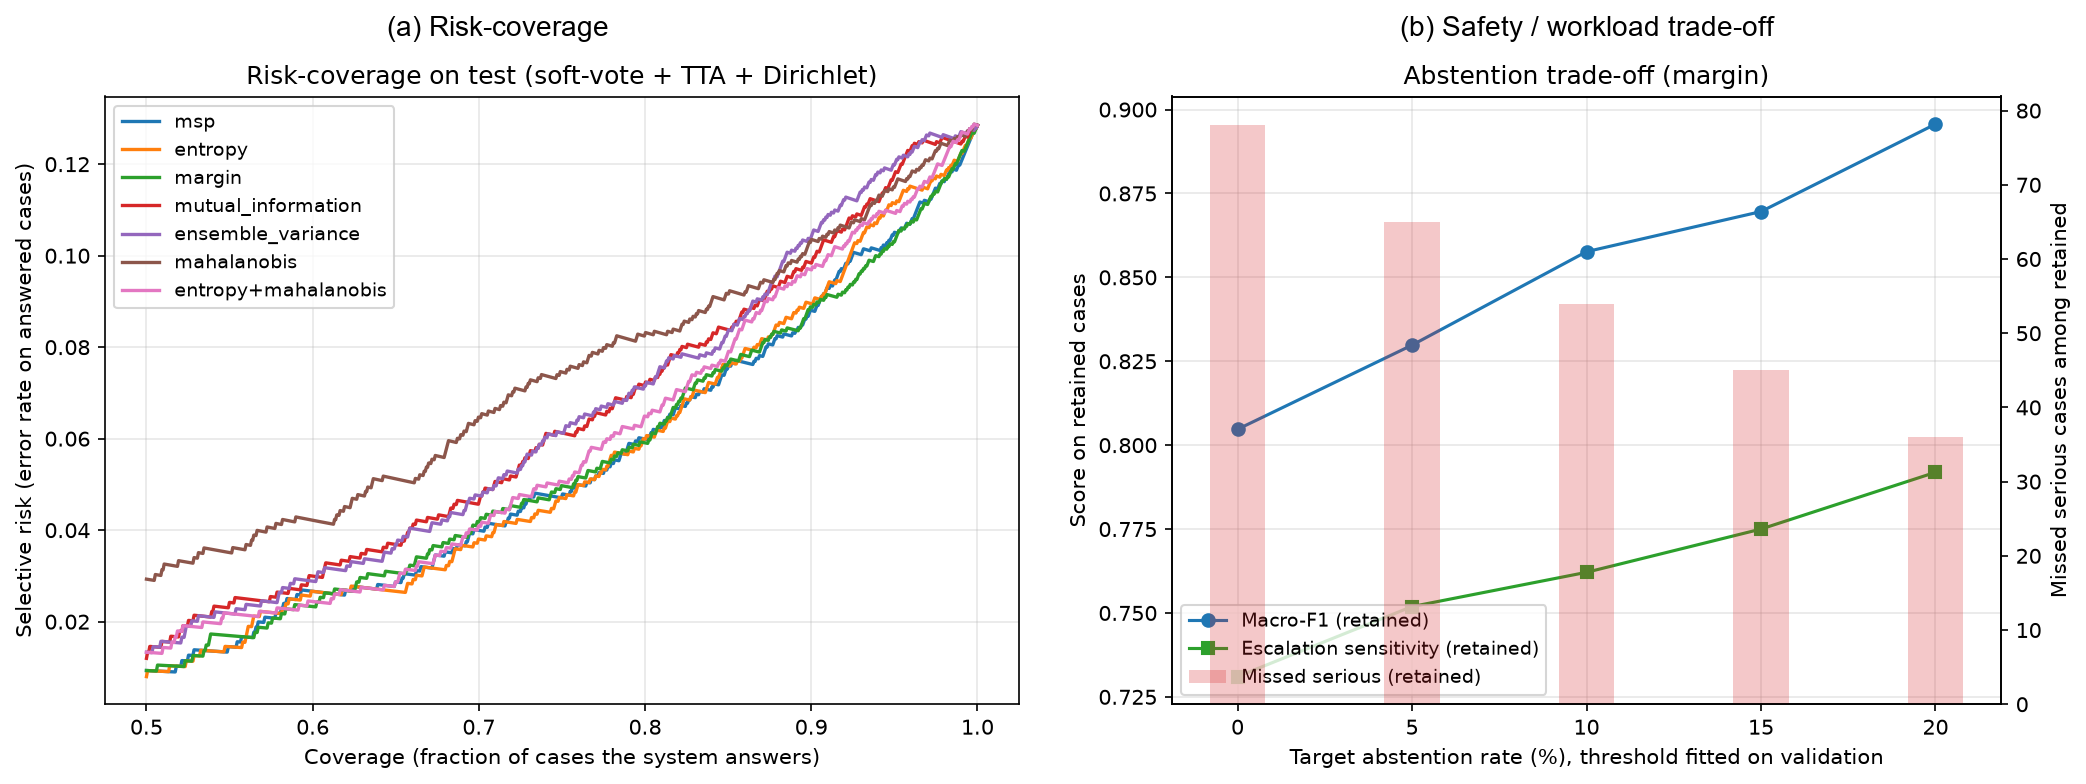
\includegraphics[width=0.86\textwidth]{figure4_selective.png}
\caption{Selective classification on the test split. \textbf{(a)} Risk--coverage curves for
the seven uncertainty scores. The three probability-based scores (margin, MSP, entropy) are
mutually indistinguishable; the disagreement-based scores (mutual information, ensemble
variance) are consistently worse, and Mahalanobis feature distance is worst by a clear
margin across the whole operating range. The margin was selected on validation AURC, but its
advantage over MSP and entropy is not resolvable on test. \textbf{(b)} The aggregate
safety/workload trade-off for the selected score: Macro-F1 and escalation sensitivity on the
retained cases rise monotonically with the deferral rate while missed serious cases fall from
$78$ to $36$. Panel~(b) is well behaved at every operating point, which is precisely why the
subgroup breakdown in Table~\ref{tab:agegap} --- and not this figure --- is what exposes the
under-$40$ failure.}
\label{fig:selective}
\end{figure*}

Ranked by validation AURC, the top-two margin wins ($0.02563$), followed by MSP
($0.02671$), entropy ($0.02714$), entropy $+$ Mahalanobis ($0.02795$), mutual information
($0.03226$), inter-member variance ($0.03371$) and Mahalanobis distance ($0.03558$). The
ordering holds on test (margin E-AURC $0.02242$; Mahalanobis $0.03097$).

\textbf{Mahalanobis distance ranks last, and this is the expected result.} Feature-space
distance answers the question ``is this input unlike anything seen in training?''. Every
image in this test split is HAM10000 dermoscopy drawn from the same acquisition process as
the training set, so there is no distribution shift for it to detect. What abstention needs
to rank here is \emph{in-distribution difficulty} --- genuinely ambiguous lesions near a
decision boundary but comfortably inside the feature manifold --- and the probability vector
measures exactly that. Consistent with this reading, combining Mahalanobis with entropy is
worse than entropy alone. We regard the Mahalanobis score as untested rather than refuted:
the honest venue for it is an out-of-distribution stream such as smartphone clinical
photography, which this split by construction does not contain.

Block B of Table~\ref{tab:ablation} gives the selective results. Deferring the $10.8\%$ of
cases with the smallest gap between their top two class probabilities raises Macro-F1 on the
retained set from $0.8047$ to $0.8577$
and cuts missed serious cases from $78$ to $54$; at $22.1\%$ deferral the retained Macro-F1
reaches $0.8957$ with $36$ missed. We emphasise that these rows have a different denominator
($1{,}340$ and $1{,}170$ images against $1{,}502$) and are not like-for-like with Block A:
the classifier is being handed an easier subset, not becoming a better classifier. This is
why they occupy a separate, coverage-annotated block, and why Fig.~\ref{fig:selective}(a)
rather than the table carries the substantive claim.

One systematic effect is worth recording. Requested abstention rates of $5/10/15/20\%$ yield
realised test coverages of $0.954/0.892/0.836/0.779$ --- roughly one percentage point more
abstention than the validation quantile promised, consistently at every operating point.
That is the expected signature of a threshold fitted on data the backbones were themselves
optimised against, and it bounds the optimism of our validation-derived operating points at
approximately one point of coverage.

\textbf{Refitting the gate out-of-fold changes which score wins, which is itself informative.}
Selecting the uncertainty score by AURC on the $6{,}981$ OOF rows rather than the $1{,}532$
validation rows promotes maximum softmax probability over the top-two margin
(Table~\ref{tab:oof_vs_val}). The two are statistically indistinguishable on test
(Fig.~\ref{fig:selective}(a)), so this is a coin landing the other way rather than a
correction; but it means the two arms' abstention thresholds live on different scales and
their numerical values are not comparable across arms. The OOF-fitted gate is the one used
for the orthogonality analysis in Sec.~\ref{sec:results-utility}, where at a $10\%$ target it
retains $89.9\%$ of cases, raises retained Macro-F1 from $0.7871$ to $0.8444$, and cuts
missed serious cases from $78$ to $57$. Substituting one probability-based score for another
does not change the paper's conclusions, and we checked specifically that it does not change
the under-$40$ finding: the confidently-wrong pattern reproduces under MSP as it does under
margin.

\subsection{Explainability}
\label{sec:results-gradcam}

\begin{figure*}[t]
\centering
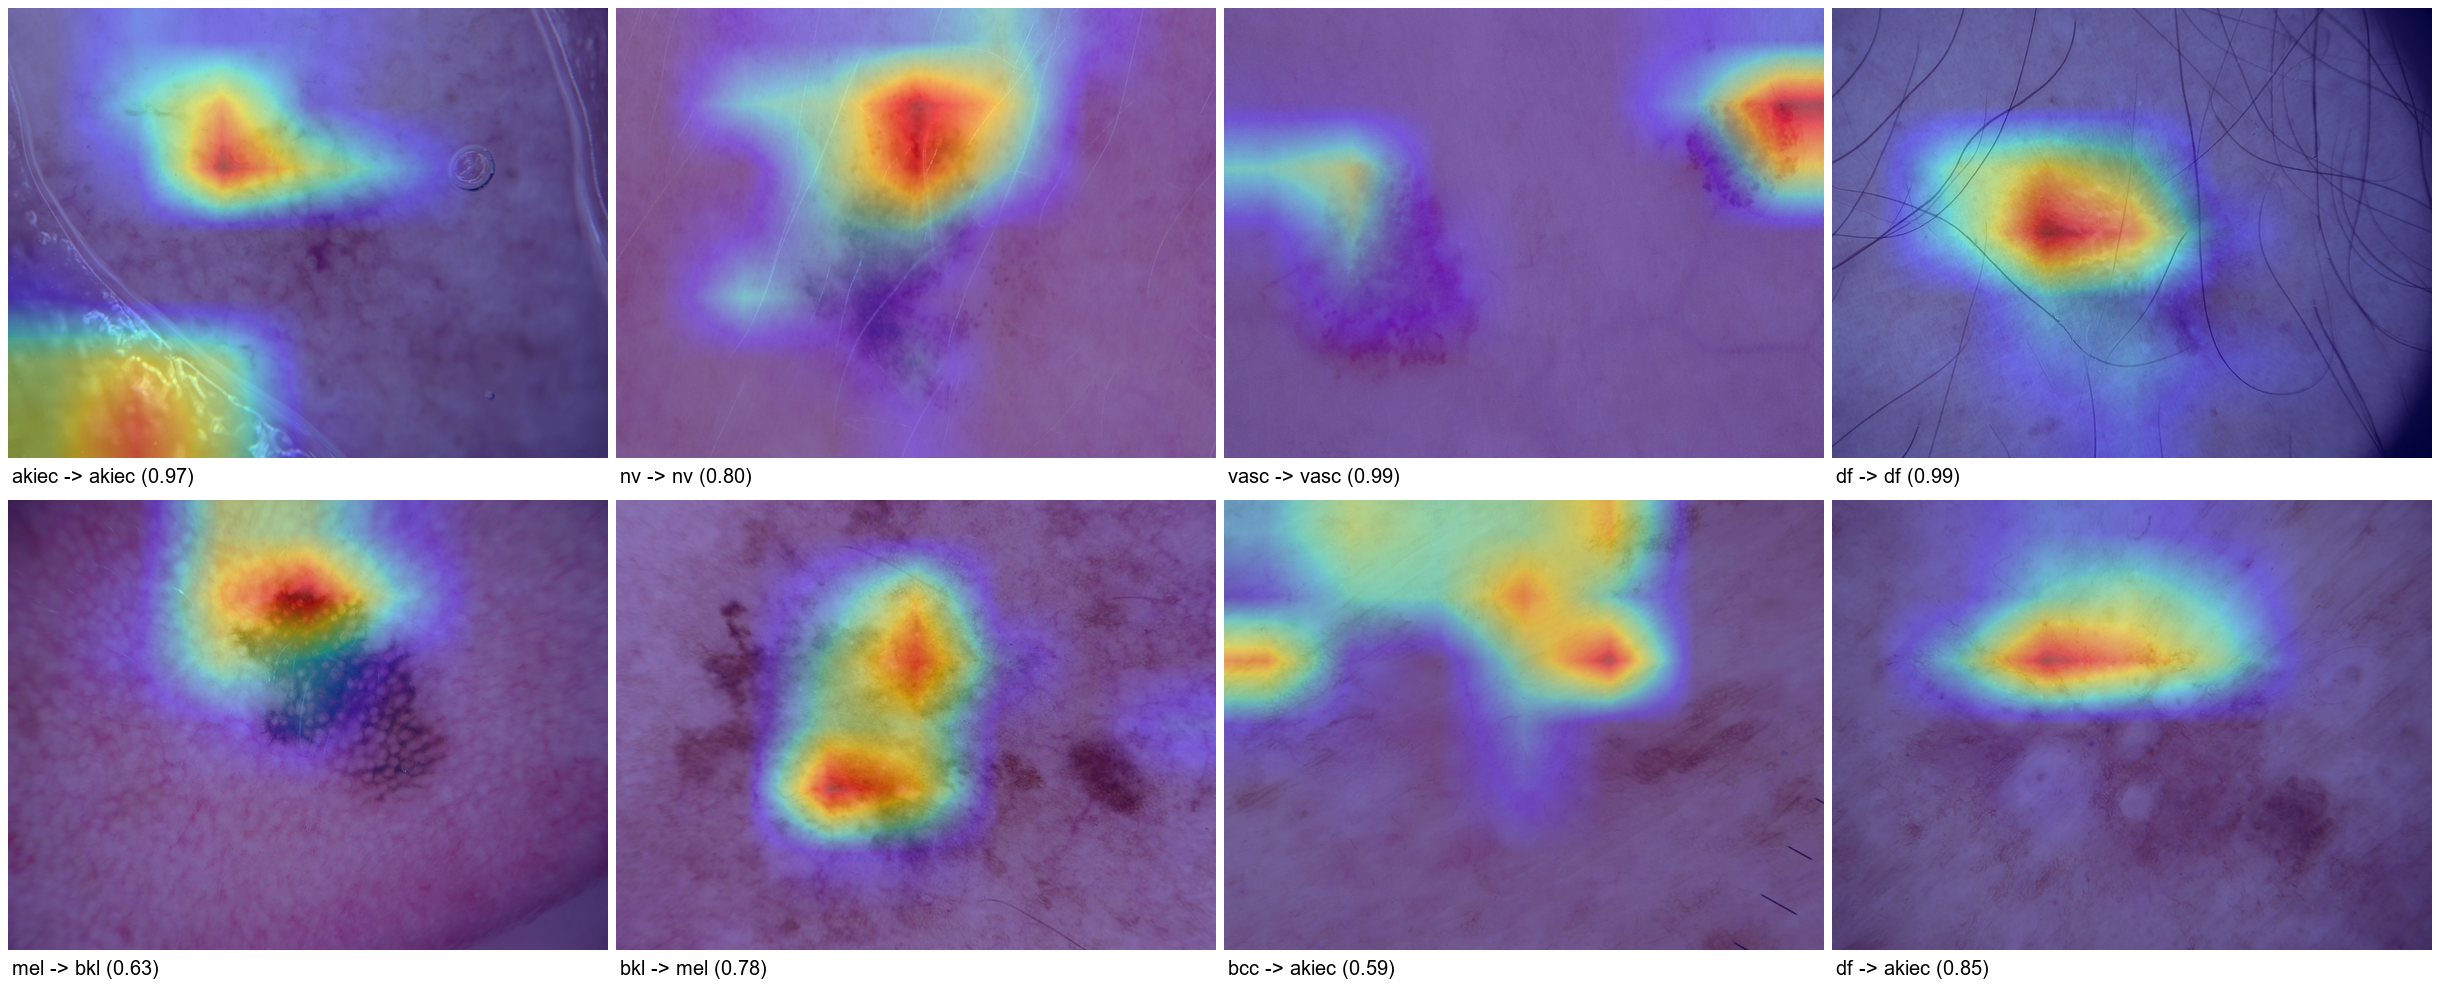
\includegraphics[width=0.90\textwidth]{figure7_gradcam.png}
\caption{Grad-CAM attributions for ConvNeXt-Tiny on the test split. Top row: the
highest-confidence correct case for four classes the model handles well. Bottom row: the
highest-confidence \emph{error} for four classes it confuses, including both directions of
the \textsc{mel}/\textsc{bkl} confusion. Each panel prints true $\rightarrow$ predicted and
the softmax value; panels are selected deterministically by confidence from
\texttt{gradcam\_stats.csv}. These are the model's \emph{most} confident errors, which at
$0.59$--$0.85$ still straddle its mean confidence of $0.7048$, so the row illustrates the
failure mode rather than quantifying it. Read the maps as illustration only: over all
$1{,}502$ test images the lesion-interior mass fraction is $0.523$, and it is \emph{higher}
for errors than for correct predictions --- a predicted-class artefact analysed in the text,
not evidence that errors are the better localised.}
\label{fig:gradcam}
\end{figure*}

Grad-CAM~\cite{selvaraju2017gradcam} overlays were generated for the ConvNeXt-Tiny model on
$28$ test images, four per class, split between correct and incorrect predictions
(Fig.~\ref{fig:gradcam}).

An earlier version of this analysis used only a \emph{border mass fraction} --- the share of
heatmap activation falling in the outer $15\%$ of the frame --- as a proxy for whether the
model was responding to vignetting rather than to the lesion. That is an image-frame
heuristic, not a lesion boundary. Using Tschandl's binary lesion segmentations for
HAM10000~\cite{tschandl2020segmentations} we can instead compute the quantity of interest
directly, over all $1{,}502$ test images with no missing mask: the fraction of Grad-CAM
activation mass falling \emph{inside} the annotated lesion. It is $0.523$ $[0.509, 0.536]$,
against a mean lesion area of $0.256$ of the frame --- a concentration ratio of $3.45$. Roughly
half the attribution mass lands on a quarter of the image, so the model is attending to the
lesion far more than area alone would predict.

We are explicit that this is a supporting check and not evidence of mechanism, for two
reasons. Saliency maps fail known sanity checks~\cite{adebayo2018sanity}. And more
specifically, the metric is confounded here in a way that is visible in our own numbers:
\emph{misclassified} images score \emph{higher} on lesion-interior fraction ($0.570$ $[0.533,
0.611]$) than correct ones ($0.513$ $[0.499, 0.528]$). That is not evidence that errors are
better localised. For a misclassified image the map is taken with respect to the
\emph{predicted} class logit, so landing on the lesion is close to automatic, and the
per-class breakdown confirms the artefact: the fraction is lowest for \textsc{nv} ($0.477$),
the class the model over-predicts. Attribution here shows \emph{where} the network looked, not
that melanoma-relevant features were extracted.

The mechanistic claim in this paper is therefore carried by the escalation-mass AUC of
Sec.~\ref{sec:results-fairness}, not by these maps. That statistic is a direct, threshold-free
measurement of whether the discriminative information survived into the probability vector,
which is the question at issue; a saliency map cannot answer it.

\subsection{Intersectional slices, and the cells we decline to report}
\label{sec:results-intersectional}

Age is not the only axis, and disparities can compound. We slice age band $\times$ sex on the
test split under the same power gates the rest of our subgroup analysis uses: at least $30$
images and at least $10$ true escalating cases before a sensitivity is reported at all. Five
of the eight cells clear both gates.

Escalation sensitivity is $0.848$ $[0.681, 0.949]$ for women aged $40$--$59$ and $0.784$
$[0.618, 0.902]$ for men in the same band; $0.697$ $[0.551, 0.833]$ for women aged $60+$ and
$0.797$ $[0.709, 0.874]$ for men. The one reportable under-$40$ cell, women, is $0.250$
$[0.055, 0.572]$ on twelve escalating lesions. Across the reportable cells the
equalised-odds true-positive-rate gap is $0.598$, the demographic-parity gap $0.339$, and the
gap in referral burden $0.129$. The dominant structure is the age gap; sex modulates it
within bands by substantially less than age separates the bands, and at these interval widths
we do not claim a resolved sex effect.

Three cells are suppressed and we name them rather than dropping them. Two hold patients with
no recorded age or sex ($n=3$ and $n=9$). The third is men under $40$: it has nine escalating
lesions against our floor of ten, so it fails the gate by one case. It is, predictably, the
cell a reader most wants to see, and it is exactly the cell at which a point estimate would be
least trustworthy; its raw counts are in the results file, and we decline to attach a
sensitivity or an interval to it here. Reporting a gate and then quietly stepping over it for
the interesting cell would defeat the purpose of having set one.

\subsection{External evaluation: smartphone clinical photography}
\label{sec:results-external}

% generated by research/external/render_composite_tables.py -- do not hand-edit
% supersedes external_table_{bcn_age_replication,pad_prior_shift,cross_cohort_triage,
%   decision_curve,conformal_shift,fitzpatrick_slices}.tex, which stay on disk as the
%   per-analysis outputs of their own scripts but are no longer part of the manuscript.
\begin{table*}[t]
\centering
\caption{Safety nets under distribution shift. Panel~(A): the shift is detectable and the conformal sets widen under it, converting silent point errors into visible uncertainty --- but coverage itself degrades sharply, and the guarantee does not survive the move. Split conformal finite-sample coverage guarantees hold under exchangeability. External cohorts (PAD-UFES-20) are by construction non-exchangeable; coverage is reported as an empirical audit of safety-net widening behavior. Panel~(B): across the 4 adequately powered strata the Tier-1 sensitivity spread is 0.067 and it is \emph{not} monotonic in Fitzpatrick type (I~0.269, II~0.203, III~0.203, IV~0.231), so these data do not reproduce the reported darker-skin penalty. Only 1{,}302 of the 2{,}106 lesions carry a Fitzpatrick label at all; the two darkest strata are suppressed at $n=8$ and $n=1$, so this cohort cannot speak to darker skin. The unlabelled remainder holds no Tier-1 lesion, so a pooled labelled-versus-unlabelled gap is a data-completeness artefact and is not reported here as a skin-tone effect.}
\label{tab:external_safety}
\footnotesize
\setlength{\tabcolsep}{4pt}
\begin{tabular}{@{}lcccccccc@{}}
\toprule
\multicolumn{9}{@{}l}{\textbf{(A) Shift detection and conformal set widening.} In-distribution reference is the HAM10000-OOF tuning half, held out from the quantile estimate; the shifted cohort is PAD-UFES-20.} \\
\addlinespace[0.2em]
\multicolumn{9}{@{}l}{\emph{Mahalanobis detector} (fit on HAM10000 train features, no refit): median score 485 in distribution against 8{,}717 under shift (18.0$\times$ separation), AUROC 0.9128.} \\
\addlinespace[0.3em]
Conformal method & \multicolumn{4}{c}{In distribution (HAM10000 OOF)} & \multicolumn{4}{c}{Under shift (PAD-UFES-20)} \\
\cmidrule(lr){2-5}\cmidrule(l{0.4em}){6-9}
 & Marginal & Serious & set-FRR & Mean $|\mathcal{C}|$ & Marginal & Serious & set-FRR & Mean $|\mathcal{C}|$ \\
\midrule
LAC marginal $\alpha=0.10$ & 0.9052 & 0.7192 & 0.2526 & 1.08 & 0.2379 & 0.1217 & 0.7462 & 1.15 \\
LAC Mondrian $\alpha=0.10$ & 0.8816 & 0.8990 & 0.0743 & 1.26 & 0.4136 & 0.3516 & 0.2747 & 2.10 \\
LAC Mondrian $\alpha=0.05$ & 0.9365 & 0.9406 & 0.0386 & 2.33 & 0.6220 & 0.5722 & 0.1057 & 3.37 \\
APS Mondrian $\alpha=0.05$ & 0.9465 & 0.9495 & 0.0297 & 2.49 & 0.6548 & 0.5907 & 0.0725 & 4.06 \\
\midrule
\multicolumn{9}{@{}l}{\textbf{(B) Fitzpatrick skin-tone strata (PAD-UFES-20).} Pre-registered reporting gates: $N \ge 30$ and $N_{\text{Tier 1}} \ge 10$. Intervals are exact Clopper--Pearson; conformal sets are Mondrian $\alpha=0.05$.} \\
\addlinespace[0.2em]
Stratum & $N$ & $N_{\text{Tier 1}}$ & Tier-1 sens.\ [95\% CI] & point-FRR & set-FRR [95\% CI] & Mean $|\mathcal{C}|$ &  &  \\
\midrule
Type I & 137 & 104 & 0.269 [0.187, 0.365] & 0.606 & 0.096 [0.047, 0.170] & 3.48 &  &  \\
Type II & 750 & 537 & 0.203 [0.170, 0.239] & 0.680 & 0.060 [0.041, 0.083] & 3.50 &  &  \\
Type III & 347 & 227 & 0.203 [0.152, 0.261] & 0.709 & 0.101 [0.065, 0.148] & 3.42 &  &  \\
Type IV & 59 & 26 & 0.231 [0.090, 0.436] & 0.615 & 0.077 [0.009, 0.251] & 3.00 &  &  \\
Type V & 8 & 3 & \multicolumn{3}{c}{\emph{suppressed: $N < 30$; $N_{\text{Tier 1}} < 10$}} & 3.38 &  &  \\
Type VI & 1 & 0 & \multicolumn{3}{c}{\emph{suppressed: $N < 30$; no Tier-1 lesion, so Tier-1 rates are undefined}} & 4.00 &  &  \\
Unlabelled / missing & 804 & 0 & \multicolumn{3}{c}{\emph{suppressed: no Tier-1 lesion, so Tier-1 rates are undefined}} & 3.31 &  &  \\
\bottomrule
\end{tabular}
\end{table*}


We finally apply the frozen system --- six backbones, the uniform vote, the HAM-fitted
Dirichlet map and the out-of-fold-fitted age rule, all unmodified --- to the external cohort
of Sec.~\ref{sec:external-data}, all $2{,}106$ PAD-UFES-20
images~\cite{pacheco2020padufes}. This follows the standard protocol for
evaluating uncertainty under dataset shift~\cite{ovadia2019shift,
lakshminarayanan2017deepensembles}. Nothing was fitted or tuned on PAD.

\textbf{The system does not transfer, and the ensemble transfers worst.} Individual members
reach Macro-F1 $0.124$--$0.188$. The uniform six-CNN soft-vote reaches $0.167$ --- \emph{below
its own best member} (ConvNeXt-Small, $0.188$). The diversity that makes ensembling the one
significant rung in-distribution disappears under domain shift, because the members' errors
become correlated: they fail on the same images for the same reason. Applying the frozen
HAM-fitted Dirichlet map on top makes matters worse still ($0.167 \rightarrow 0.130$,
escalation sensitivity $0.356 \rightarrow 0.221$), which is the expected behaviour of a
calibration map transported to a distribution whose class prior is inverted. Nothing in this
paper licenses pointing a dermoscopy-trained classifier at phone photographs.

\textbf{How much of that collapse is the prior, and how much is the optics?} Panel~B of
Table~\ref{tab:external_battery} decomposes it. The system's implicit source prior --- the
mean of its own predictions over the out-of-fold panel --- is $\textsc{nv}\ 0.510$,
$\textsc{mel}\ 0.100$, $\textsc{bcc}\ 0.069$; PAD's true prior is close to its inverse
($\textsc{bcc}\ 0.401$, $\textsc{akiec}\ 0.347$, $\textsc{nv}\ 0.116$). Handed PAD's true
class frequencies, the same frozen network reaches Macro-F1 $0.253$ against $0.167$ raw, a
$52\%$ relative gain: prior shift is a real and substantial part of the failure. It is not
most of it. An oracle that is told the answer still lands at $0.253$, so the majority of the
gap is optical --- the features themselves change when polarised dermoscopy becomes a phone
camera, and no reweighting recovers that. The deployable version of the correction is worse
than useless. Saerens EM~\cite{saerens2002adjusting}, which estimates the target prior
without labels, converges in $109$ iterations to $\textsc{df}\ 0.481$ where the truth is
$0.000$ and $\textsc{bcc}\ 0.125$ where the truth is $0.401$, and Macro-F1 falls to $0.102$.
Its pre-registered confirmatory test is significant \emph{in the wrong direction}
($\chi^2 = 98.73$, $p = 2.89\times10^{-23}$; $321$ cases are correct only without the
correction against $113$ only with it). EM assumes the class-conditional likelihoods survive
the shift. Here they do not, so the algorithm converges to a fixed point that is internally
consistent with the model's beliefs and externally wrong --- a useful negative result, since
label-free prior correction is the obvious thing a deployer would reach for.

\textbf{The age rule does no harm and plausibly helps, but this is not a replication and we
will not call it one.} Applied on top, the frozen $\lambda$ lifts escalation sensitivity from
$0.221$ to $0.568$, melanoma recall from $0.115$ to $0.327$, missed serious cases from
$1{,}268$ to $703$, and Macro-F1 from $0.130$ to $0.172$. Read carelessly this looks like
external validation of the mitigation. It is not. PAD's escalating prevalence is
approximately $77\%$, the \emph{inverse} of HAM10000's $19\%$, so a constant additive bonus on
escalating classes must help mechanically under this prior shift, whether or not the specific
under-$40$ mechanism we identified is what is firing. We report it as a directional,
non-pre-registered probe showing the intervention causes no harm and plausibly helps under
extreme prior shift --- strictly weaker evidence than a same-modality replication, which
remains outstanding. And even with the rule, Macro-F1 ($0.172$) stays below the best raw
single member ($0.188$): PAD is a different domain, not a rescued deployment.

\textbf{Mahalanobis distance, given the shift it was designed for, works, and the conformal
sets widen when it fires.} Ranked last of seven uncertainty scores on the in-distribution
test split (Sec.~\ref{sec:results-selective}), the same class-conditional Mahalanobis score
--- fitted on HAM training features and not refitted --- separates in-distribution HAM
validation ($n=1{,}532$) from shifted PAD ($n=2{,}106$) at AUROC $0.913$, with median scores
of $485$ against $8{,}717$, an $18\times$ separation
(Table~\ref{tab:external_safety}, panel~A). Its in-distribution failure was not a defect of
the score but a mis-specified task: there was no shift to detect. The two results together
are the argument for pairing a boundary-based score for in-distribution abstention with a
density-based score for shift detection, rather than choosing between them. The same panel
audits what the conformal machinery does under that shift, and the answer is two-sided: the
sets widen as they should --- APS-Mondrian at $\alpha=0.05$ goes from a mean $2.49$ labels in
distribution to $4.06$ under shift, and its singleton rate collapses from $0.141$ to $0.035$,
so silent point errors become visible ambiguity --- but serious-class coverage still falls
from $0.950$ to $0.591$. Widening is a warning light, not a guarantee. Nothing about
exchangeability survives a change of imaging modality, and we report the external coverage as
an empirical audit with no finite-sample claim attached.

\textbf{Skin tone: what PAD can and cannot say.} PAD carries a Fitzpatrick label for $1{,}302$
of $2{,}106$ images. Four types clear our power gate --- I ($n=137$), II ($750$), III ($347$),
IV ($59$) --- and types V ($8$) and VI ($1$) do not, and are reported as suppressed. A pooled
equalised-odds true-positive-rate gap across all groups is $0.295$, but that figure is
\emph{not} a skin-tone finding and must not be quoted as one: it is driven almost entirely by
the $804$ images with no Fitzpatrick label, whose escalation sensitivity is $0.054$ against
$0.247$--$0.349$ for every labelled type. That is a data-completeness artefact, and the
population with missing labels differs systematically from the population with them.
Restricted to types I--IV, the true skin-tone spread is $0.102$ and \emph{non-monotonic}
(I $0.349$, II $0.287$, III $0.247$, IV $0.278$). Panel~B of
Table~\ref{tab:external_safety} reports the same four strata under the three-tier triage
taxonomy instead, where the quantity is Tier-1 sensitivity rather than escalation
sensitivity --- a narrower positive class, so the values are lower (I $0.269$, II $0.203$,
III $0.203$, IV $0.231$) --- and the conclusion is the same one: a spread of $0.067$, and
still non-monotonic. The unlabelled stratum contains no Tier-1 lesion at all, which is why
its Tier-1 rates are reported as undefined there rather than as zero, and why the pooled gap
is a statement about which lesions get a Fitzpatrick record, not about skin tone. It does not
reproduce the
darker-skin-underperforms pattern reported elsewhere in dermatological
AI~\cite{daneshjou2022disparities}, and we do not read that as evidence of absence: $n=59$ at
type IV is thin and types V and VI are effectively absent from the cohort. The honest summary
is that this evaluation closes the skin-tone question for types I--IV on smartphone
photography and leaves it open for darker skin, which requires a corpus that
contains it~\cite{groh2021fitzpatrick17k}.


\section{Extended Discussion}
\label{app:extdiscussion}

\subsection{What actually moved the needle, and what did not}
Across a ladder spanning two architecture families, two imbalance-targeted losses, metadata
fusion, ensembling, TTA, calibration, thresholding and abstention, exactly one design choice
produced a gain this test split can certify: ensembling (McNemar Holm-adjusted
$p=2.0\times10^{-4}$; DeLong on \textsc{bkl} AUC, Holm-adjusted $p=0.013$). Every other rung
is a consistent, and from A5 onward a monotone, improvement that remains individually
unresolvable at this sample size.

We then went looking for more, and did not find it. Five further combination levers --- adding
two transformer members, greedy member selection, global prior correction, per-class offsets,
and a $30$-member fold-bagged ensemble --- were fitted and selected without touching test, and
all five came back negative (Sec.~\ref{sec:results-exhaustion}). The last of them,
fold-bagging --- the only one with a real mechanism behind it --- was named in the analysis
plan before it existed and read once, alongside its companion calibration rung A7-oof, which
is also negative. We take
two lessons. First, single-split comparisons of architectures on HAM10000 have exhausted their
informational content, and papers reporting one- to three-point Macro-F1 improvements without
interval estimates or paired tests are reporting sampling noise. Second, and more usefully:
the interesting axis of variation has moved from \emph{how accurate} to \emph{how usable}. The
gap between a raw ensemble and one that is calibrated, knows when to abstain, and emits
prediction sets that are valid \emph{for the patient in front of you} is far larger, in terms
of what a clinician can act on, than any architectural gap we measured.


% From here the checklists need \onecolumn: longtable cannot break across a
% two-column page. Nothing below declares a starred float.
\clearpage
\onecolumn
\input{tables/appendix_checklists.tex}

\end{document}
